%##################################################################################
\documentclass[enabledeprecatedfontcommands,12pt,a4paper,twoside,hyphens]{scrreprt}
%\documentclass[enabledeprecatedfontcommands,12pt,a4paper,twoside,hyphens]{scrreprt}

\usepackage[utf8]{inputenc}

\usepackage{graphicx}
\usepackage{pdfpages}


 % Neue deutsche Rechtschreibung und Silbentrennung.
\usepackage[ngerman]{babel}

%%europäische Schriftzeichen (ä,ö)
\usepackage[T1]{fontenc}

%%Mathepages
\usepackage{amsfonts}
\usepackage{amsmath}


%%Fallbetrachtungen
\usepackage{cases}
%Algorithmus
\usepackage[ruled,vlined]{algorithm2e}

\usepackage[noend]{algpseudocode}
%\usepackage{arevmath} 	%math symbols
%\usepackage[]{algorithm}
\usepackage{amsmath}

\usepackage{lipsum, todonotes}	
\usepackage[nolist,nohyperlinks]{acronym}
\usepackage{caption}
\usepackage{float}

%%Tabellen Packages
\usepackage{multirow}
\usepackage{booktabs}

%%Erstekken von Listen 
\usepackage{listings}

%Acronyme
\usepackage{acronym} 

%an klickbare links in der PDF
\usepackage{hyperref}
\usepackage[sf]{titlesec}            

% Header and Foot
\usepackage{fancyhdr}

\usepackage{setspace}
\linespread{1.25}

%Leerseite
\usepackage{afterpage}

%\newboolean{titel} 
%\setboolean{titel}{true}
%\newboolean{inhalt} 
%\setboolean{inhalt}{true}
%\newboolean{headfoot} 
%\setboolean{headfoot}{true}

% Dokumentangaben
\newcommand{\dokumenttitel}{[Genetische Algorithmen zur
Optimierung von Hyperparametern eines
künstlichen neuronalen Netzes]}
\newcommand{\untertitel}{[Untertitel]}
\newcommand{\version}{0.1}
\newcommand{\veroeffentlichung}{21.01.2020}
\newcommand{\autor}{[Christian Heinzmann]}
\newcommand{\state}{-vertraulich-}

%Titelseite?
%\setboolean{titel}{false} 
%Inhaltsverzeichnis?
%\setboolean{inhalt}{false}
%FZI Kopf- und Fußzeile?
%\setboolean{headfoot}{false}

%Inhaltsverzeichnis?
%\setboolean{inhalt}{false}
%FZI Kopf- und Fußzeile?
%\setboolean{headfoot}{false}

\setcounter{tocdepth}{1}
\begin{document}

\pagestyle{empty}


\includepdf[pages=-,offset=-0ex -0ex]{Titelblatt.pdf}





\newcommand\blankpage{%
    \null
    \thispagestyle{empty}%
    \addtocounter{page}{-1}%
    \newpage}
    
\afterpage{\blankpage}
\afterpage{\blankpage}
\afterpage{\blankpage}


\cfoot{}

\pagestyle{fancy}
\fancyhf{}

\fancyhead[LO]{\sf{\rightmark}}
\fancyhead[RE]{\sf{\leftmark}}

\fancyfoot{}
\fancyfoot[LO,RE]{\thepage}

\fancypagestyle{plain}{
    \fancyhf{}
    \fancyfoot[LO,RE]{\thepage}
    %\fancyhf{}
    \renewcommand{\headrulewidth}{0pt}
}

\pagenumbering{roman}
\setcounter{page}{1}
\addsec{Eigenständigkeitserklärung und Hinweis auf verwendete
Hilfsmittel}
\label{erklaerung}

Eigenständigkeitserklärung und Hinweis auf verwendete
Hilfsmittel.
Hiermit bestätige ich, dass ich den vorliegenden Praxissemesterbericht selbständig
verfasst und keine anderen als die angegebenen Hilfsmittel benutzt habe. Die Stellen
des Berichts, die dem Wortlaut oder dem Sinn nach anderen Werken entnommen sind,
wurden unter Angabe der Quelle kenntlich gemacht.\\
\\[1.5cm]
Datum:	\hrulefill\enspace Unterschrift: \hrulefill
\\[3.5cm]



\cleardoublepage

\chapter*{Kurzfassung}
\chapter*{Kurzfassung}
\label{sec:Kurzfasssung}
Im Kontext der Klassifizierung von Aktion und Objekten, soll die Optimierung von Hyperparametern bei künstlichen neuronalen Netzen mit Hilfe von Genetischen Algorithmen im Rahmen dieser Arbeit durchgeführt werden. Da es für die Hyperparameter keine klaren Regeln gibt und sie je nach Daten und Modell-Architektur anders gewählt werden müssen. Somit ist es für den Entwickler sehr zeitaufwendig, diese Hyperparameter von Hand auszuwählen. Daher ist das Ziel der Arbeit, ein Framework zu entwickeln und zu implementieren, in dem künstliche neuronale Netze automatisiert trainiert, getestet, Hyperparameter angepasst und ausgewertet werden. Dazu wurde ein Konzept entwickelt, in welchem die Hyperparameter als Gene des Genetischen Algorithmus umgesetzt werden. So werden die Hyperparameter nach dem Vorbild der Evolution über Generationen intelligent angepasst. Des Weiteren wurde der State-of-the-Art Algorithmus ausgesucht und implementiert, um den Genetischen Algorithmus vergleichen zu können. Es handelt sich um die Zufallssuche, welche zufällige Individuen im Suchraum testet. Beide Optimierungsalgorithmen wurden zur Optimierung von Hyperparametern in Fully Connected Networks und Convolutional Neural Networks verwendet. Zudem wurden verschiedene Datensätze verwendet, um eine unabhängige Aussage zu erreichen. Der Genetische Algorithmus konnte leider keine Verbesserungen im Vergleich zur Zufallssuche erreichen. Beide Algorithmen finden Hyperparameter, welche gleich gute Klassifizierungsergebnisse liefern. Sie unterscheiden sich nur im Nachkommabereich und sind somit vernachlässigbar klein. Dennoch hat der Genetische Algorithmus einen Vorteil: Über seine letzte Population kann eine zusätzliche Aussage getroffen werden, in welchem Bereich sich die Hyperparameter befinden müssen, um gute Ergebnisse zu erreichen. Dies ist mit der Zufallssuche nicht möglich, da diese nicht genügend gute Individuen findet, um diese Aussage zu treffen. Die wenigen die die Zufallssuche findet, sind ausreichend gut und können von dem Genetischen Algorithmus nicht übertroffen werden.
\cleardoubleoddpage

% Beendet eine Seite und erzwingt auf den nachfolgenden Seiten die Ausgabe aller Gleitobjekte (z.B. Abbildungen), die bislang definiert, aber noch nicht ausgegeben wurden. Dieser Befehl fügt, falls nötig, eine leere Seite ein, sodaß die nächste Seite nach den Gleitobjekten eine ungerade Seitennummer hat. 


%Inhaltsverzeichnis
\tableofcontents
\cleardoublepage


\normalsize
\pagenumbering{arabic}
\setcounter{page}{1}

\chapter{Einleitung}
%\chapter{Einleitung}

\section{Einleitung zum Forschungs Zentrum Informatik}
\label{sec:FZI}
\glqq Das FZI Forschungszentrum Informatik am Karlsruher Institut für Technologie ist eine gemeinnützige Einrichtung für Informatik-Anwendungsforschung und Technologietransfer. Es bringt die neuesten wissenschaftlichen Erkenntnisse der Informationstechnologie in Unternehmen und öffentliche Einrichtungen und qualifiziert junge Menschen für eine akademische und wirtschaftliche Karriere oder den Sprung in die Selbstständigkeit.\grqq{} \cite{FZI_info}

\section{Der FZI-Forschungsbereich ESS}
\label{sec:ESS}
\glqq Der Forschungsbereich \acf{ESS} beschäftigt sich mit innovativen Technologien, Entwurfsmethoden und Anwendungen für und von eingebetteten Systemen. Von modellbasierten Entwurfsmethoden und -werkzeugen über technologieorientierte Forschung bis hin zu anwendungsorientierten Forschungs- und Entwicklungsprojekten – wir gestalten und entwickeln praxistaugliche Anwendungen rund um eingebettete Systeme und evaluieren diese.

Die breite Technologie- und Systemkompetenz aus Elektronik, Software-Engineering, Optik und Optoelektronik, Mikrosystemtechnik und Sensorik ist ein Alleinstellungsmerkmal des Bereiches. Schwerpunkte der Arbeiten bilden dementsprechend vor allem stark interdisziplinäre, Technologieübergreifende Forschungsprojekte und Anwendungen von eingebetteten Systemen in der Automobilelektronik, der Industrieautomation und im Gesundheits- und Sozialwesen.

Der Bereich ESS deckt mit seinen verfügbaren Kompetenzen dabei das komplette Spektrum der Entwicklung eingebetteter Systeme und Cyber Physical Systems (CPS) mit heterogenen Komponenten aus Mikroelektronik, Mikrooptik, Mikromechanik und Telematik ab.\grqq{}  \cite{ESS}




\newpage
\section{Einleitung zum Projekt}
\label{sec:Porjekt}

"Nach einer Studie der Charité aus dem Jahr 2015 sterben in Europa jährlich 23.000 Menschen an den Folgen einer Infektion mit multiresistenten Keimen. Die Tendenz ist dabei steigend. Hauptursache für die Ausbreitung dieser Keime, wie beispielsweise MRSA, ist eine mangelnde Hygiene der Angestellten in den Versorgungseinrichtungen beim Umgang mit den Patienten. Gründe dafür liegen im fehlenden Problembewusstsein, der zu hohen Arbeitsdichte und damit verbundenem Zeitmangel und der mangelnden Qualifikation der beteiligten Pflegekräfte.
\\

Ziel des Projekts HEIKE ist es neue, technikgestütze Möglichkeiten zu entwickeln, welche die behandelnden Mitarbeiter im Krankenhausumfeld bei Maßnahmen am Patienten unterstützen und dadurch deren Compliance in Bezug auf die Händedesinfektion erhöhen.
\\

Die Grundlage bilden ein mobiler, vernetzter Desinfektionsspender sowie Augmented-Reality-Technik. Die Technologien werden in dem Projekt weiterentwickelt und in einem System integriert, welches automatisch die durchgeführten Handlungen am Patienten erkennt und basierend darauf zusätzliche Informationen zur Verfügung stellt. Schließlich werden die durchgeführten Maßnahmen automatisch im System dokumentiert, was den Verwaltungsoverhead für das operative Personal verringert." \cite{FZI_Projekt}


\newpage
\section{Meine Aufgaben}
\label{sec:Aufgaben}
\begin{figure}[htb]
  \centering  
  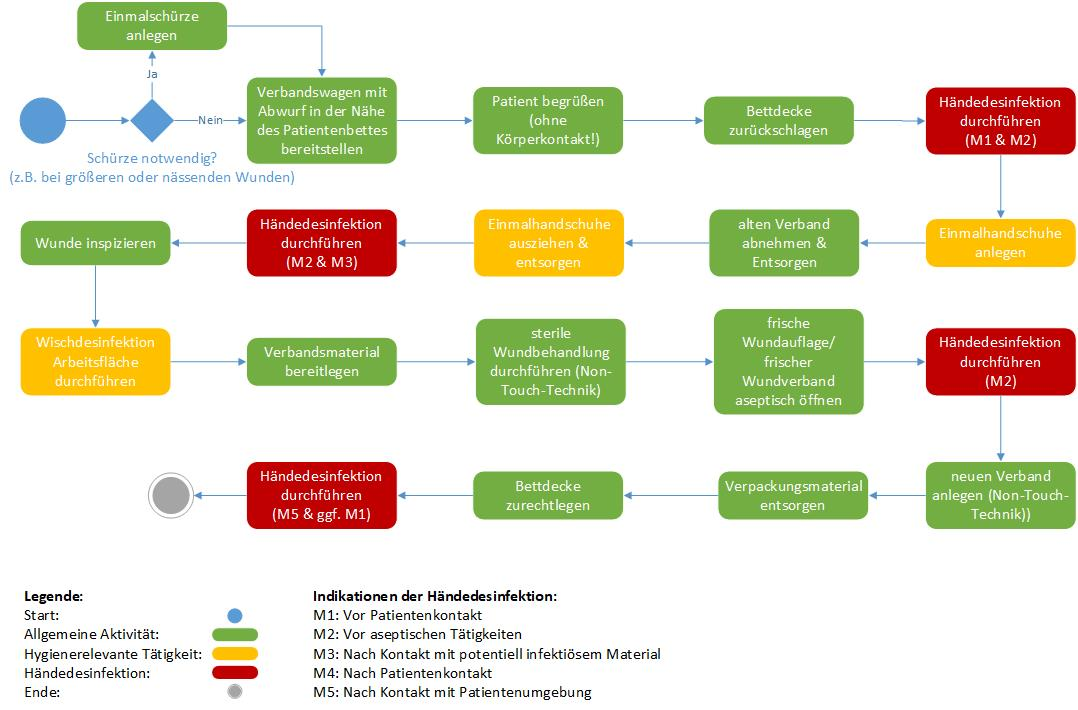
\includegraphics[scale=0.5]{img/Ablaufdiagramm_Verbandswechsel.jpg}
  \caption{Ablaufdiagramm Verbandswechsel \cite{AblauffdiagrammVerbandswechsel}}
  \label{fig:Ablaufdiagramm Verbandswechsel}
\end{figure}

Nun war die Aufgabe herrauszufinden, welche Möglichkeiten es gibt, diese Aktionen, die per EGO-Perspektiv-Video der Hololens aufgenommen wurden, zu erkennen. Die Wichtigsten Actionen sind hierbei das Desinfizieren und anlegen der Handschuhe. \ref{fig:Ablaufdiagramm Verbandswechsel}
Hierfür soll ein \acf{KNN} zuhilfe gezogen werden, welches die wichtigen Aktionen erkennt und somit die Fehlerquote, welche durch Vergessen oder Zeitstress entstehen, zu reduzieren. Dazu muss erst ein  Netz, welches für unser Anwendung passt, gefunden und für die oben genannten Anwendungen getestet werden, desweiten muss hierfür ein Datenset mit diesen Aktionen erstellt werden, welche zum Trainieren und Zesten des Netzes notwenig sind. Anschließend soll das Netz noch evaluieren und Verbesserungen vorgenommen werden.
\cleardoublepage

\chapter{Grundlagen}
\section{Grundlagen}
\label{sec:Grundlagen}
In diesem Kapitel werden die theoretischen Grundlagen, die zum Verständnis, der vorliegende Arbeit wichtig sind beschrieben. Zubeginn erfolgt eine kurzer einstieg in die Optimierungsgrundlagen. Dann folgt die Einführung in die Grundlagen der genetischen Algorithmen. Anschließend werden die wichtigen Grundlagen der Künstlichen neuronalen Netzen erklärt. Zum Schluss wird kurz auf die Hyperparameter eingegangen.

\subsection{Optimierungsgrundlagen}
Angenommen es soll ein Künstliches Neuronales Netz mit k Layern und L Neuronen zur Klassifizierung von einfachen handgeschriebenen Zahlen erstellt werden. Der Entwickler entscheidet sich für ein 3 Layern Netz mit jeweils 3 Neuronen. Nach dem Training hat es die Genauigkeit von 85 Prozent. Ist dies Akzeptabel? Kann man sagen, das für k = 3 bzw. j = 3 die optimale Lösung gefunden wurde? Um dies zu beurteilen müssen viele Experimente durchgeführt werden. Die Frage ist, wie man den die besten Werte für k und j finden um die Klassifizierung zu maximieren. Dieser Vorgang wird als Hyperparameter-Optimierung bezeichnet. Bei der Optimisierung wird mit einem Inizialwert gestartet dieser ist in den seltensten Fällen die exacte Lösung. Dieser Inizialwert muss einige male verändert werden um auf einen Optimum zu kommen. Manchmal ist dieses Anpassen/optimieren so Komplex, dass es durch eine Funktion ersetz werden muss.


\subsection{Genetische Algorithmen}

Die Inhalte des folgenden Abschnittes sind, sofern nicht anderweitig angeführt aus den Gurndlagen büchern xxxx und xxxx übernommen. 

Genetische Algorithmen sind heuristische Suchansätze. Im wesentliche zeichnet sie eine probabilistische Eltern Selektion als primären Suchoperator aus. Als Weitern Suchoperator kann noch auf die Mutation zurückgegriffen werden, dieser garantiert eine Erreichbarkeit aller Punkte im Suchraum und erhält die Grunddiversität in der Population. Es gibt zwei verschiedene Algorithmen der Standart-GA tauscht nach einer Generation die komplette Elternpopulation durch die Kinderpopulation aus. Und bestehen in der Regel immer aus fünf gleichen Schritten wie in Abb. \ref{fig:Ablauf_kurz} zusehen ist. Im Gegensatz dazu gibt es den Steady-State-GA welcher durch seine überlappende Population auszeichnet, dieser Algorithmus wird in der Arbeit nicht verwendet und wird deswegen nicht weiter erklärt. 

\noindent%
\begin{figure}[H]
  \centering  
  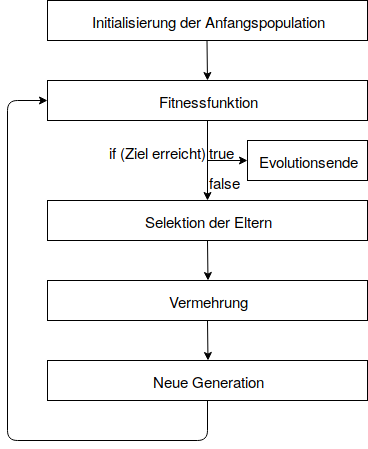
\includegraphics[scale=0.5]{img/Ablauf_kurz.png}
  \caption{Ablaufdiagramm eines Genetischen Algorithmuses mit 5 Schritten}
  \label{fig:Ablauf_kurz}
\end{figure}

Der Standard genetische Algorithmus \ref{fig:Ablauf_kurz} besteht aus folgenden 5 Schritte:
Schritt 1, Initialisieren einer Population.
Schritt 2, Fitness berechnen mit Hilfe der Fitnessfunktion.
Schritt 3, Selektieren der Eltern.
Schritt 4, Vermehren durch Cross-over und Mutation.
Schritt 5, Austausch der Populationen.
In den nachfolgenden Unterkapiteln werden auf die einzelnen Schritte genauer eingegangen. 

\iffalse
oder 

Der Standart Genetische Algortithmus \ref{Alorthm 1}besteht meist aus immer den gleichen Schritte:
Schritt 1 Inizialisieren einer Population.
Schritt 2 Fittness brechnen mit hilfe der Fitnessfunktion.
Schritt 3 Evolution (Weiterentwicken), hier werden zuerst die passenden Eltern ausgesucht und anschließend mit Crossover und Mutation die Kinder Population erstellt. 
Schritt 4 Elternpopulation durch die neue Kinderpopulation ausgetauscht.
Hier noch einamal als Pseudocode.


Algorithm 1 Basic Genetic Algorithm \\
1: initialize population \\
2: repeat \\
3: 		repeat \\
4:			fitness computation \\
5:			parent selection \\
6:			breed \\
7:		until population complete \\
8:		selection of parental population \\
9: until termination condition \\

Im nachfolgenden Unterkaptitel wird auf diese einzelnen Schritte genauer eingegangen.

\fi

\iffalse
Genetische Algorithmen sind im Wesentlichen durch eine probabilistische Eltern selektion und die Rekombination als primären Suchoperator gekennzeichnet.Die Mutation ist meist nur ein Hintergrundoperator, der mit einer geringen Wahrschenlichkeit zur anwendungkommt. Er garantiert die Erreichbarkeit aller Punkte im Suchraum und erhält eine Drunddiversitöt in der Population.

Evolutionäre Algo -- s.128


Genetische Algorithmen sind heuristische Suchansätzem, die auf einer breitenbasis von Optimierungsproblemen angewendet werden können. Diese Flexibiliät macht sie für die Praxis für viele sehr attraktiv.Die Evulution ist Grundlage des Genetischen Aglorithmuses. durch die aktuelle Vielfalt und der Erfolg der Arten ist dies schon alleine ein guter Grund sich diesen Optimierungs Algortihmus näher anzuschauen. Denn sdiese Arten sind in der lage sich an ihre Umgebung anzupassen und sich zu zu komplexen Strukturen zuentwickelen, und somit das überleben in verschiedesten Umgebungen eröglichen. Hierbei ist die Paarung und Entwicklung von Nachkommen eine der Hauptprinipen des Erfolges der Evolution. In diesem Kapitel werden wir die Grundlage der GEnetischen Algorithmen näher anzuschauen. Beginnen wir mit der grundlage das es sich bei den Genetischen Algorithmen um einen Polulations ansatz handelt. Anschließend wird auf die wichtigesten genetischen Operatioren vorstellen darunter gehöhren, Selektion, Crossover und Muttation

Seite - 11 Genetic Algorithm Essentials


Algorithmus 1 zeigt den Pseudocode des grundlegenden genetischen Algorithmus, der Folgendes kann dienen als Blaupause für viele verwandte Ansätze. Am Anfang eine Reihe von Lösungen,die als Population bezeichnet wird, wird initialisiert. Diese Initialisierung wird empfohlen.um zufällig den gesamten Lösungsraum abzudecken oder um Experten zu modellieren und einzubinden. Wissen. Die Darstellung bestimmt den Initialisierungsprozess. Für BitfolgeDarstellungen ist eine zufällige Kombination von Nullen und Einsen sinnvoll, z.B.das anfängliche Zufallschromosom 1001001001001 als typische Bitfolge der Länge 10. Der Hauptgenerationskreislauf des Genetischen Algorithmus erzeugt neue Nachkommen.Kandidatenlösungen mit Crossover und Mutation, bis die Bevölkerung vollständig ist.

Algorithm 1 Basic Genetic Algorithm
1: initialize population
2: repeat
3: 		repeat
4:			fitness computation
5:			crossover
6:			mutation
7:			phenotype mapping
8:		until population complete
9:		selection of parental population
10: until termination condition

Seite - 11 Genetic Algorithm Essentials
\fi 

\subsubsection{Aufbau und Initzialisierung einer Population}
Der klassische genetische Algorithmus basiert auf einer Reihe von Kandidatenlösungen. Die Größe der Population ist somit auch die Anzahl der Lösungen. Jede Lösung kann als einzelnes Individuum gesehen werden und wird durch ein Chromosomenstrang repräsentiert. Ein Chromosom besteht wiederum aus vielen Genen, welche die Parameter/hyperparameter repräsentieren. Der Aufbau ist grafisch in Figure \ref{fig:chromosome} gut zu erkennen. Es gibt verschiedene Möglichkeiten, diese Gene dazustellen. Wie Binär oder dezimal, um die Grundlagen nahe des später folgenden Konzepts zuhalten, wird der Ablauf per Dezimal-Genen erklärt.


\iffalse
Figure \ref{fig:chromosome} veranschaulicht ein Beispiel, wie eine Population aus vier Individuen(chromosomes)mit je einem Chromosom. Ein Chromso, besitzt wiederum  vier gene. Jedes dieser Gene ist durch eine binären zahl repräsentiert. 

\fi

\noindent%
\begin{figure}[H]
  \centering  
  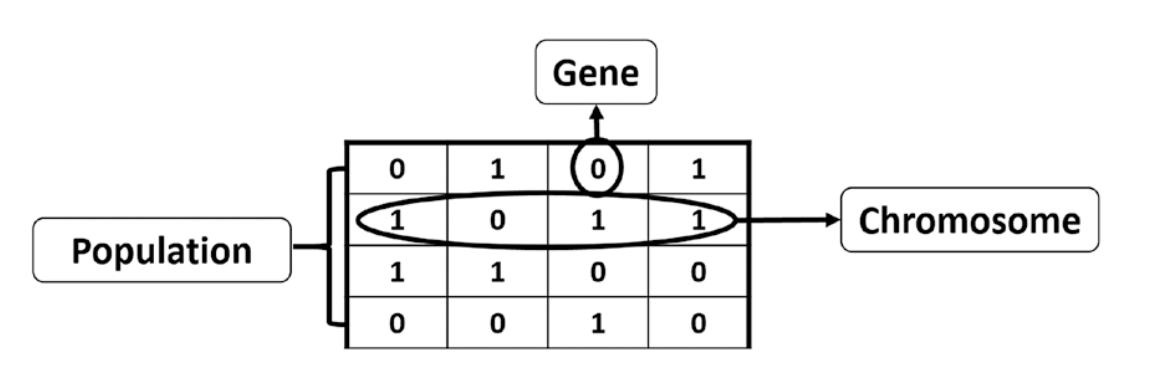
\includegraphics[scale=0.3]{img/Chromsome-s134-PracticalComputerVion.png}
  \caption{Beispiel einer Polulation mit 4 induviduen (Chromsomen) welche vier binäre Gene besitzen \cite{Rashid2017} }
  \label{fig:chromosome}
\end{figure}

Diese Anfangspopulation(Generation 0) wird zufällig initialisiert, um die größt mögliche Abdeckung des Suchraums zu gewähren. 

Die erste Generation besitzt (dadurch) eine sehr geringe Fitness, dies verbessert sich aber im Lauf des Trainings.
Die erste Generation besitzt eine sehr geringe Fittnes, welche im verlauf des Trainings stetig steigert bis sie das Maximum erreicht.

--- würde ich weglassen
Durch Selection werde die nicht unnötigen/Contra-produktiven Individumen oder auch Unfittesten Inidividuen aussotiert.
Dafür wird die Fittneswert benötig, welches im nächsten Punkt erklärt wird.
----


\subsubsection{Fittnesfunktion (eng. Fittnesfunction or grade)}
Die Fitnessfunktion bewertet das Individuum anhand seiner Funktionstauglichkeit, bezogen auf die vorhandene Aufgabe. Dabei werden nicht einzelnen Gene bewertet, sondern das ganze Genom/Chromosom/Individuum. Es gibt keine universelle Fitnessfunktion, diese muss also für jede Anwendung speziell geschrieben werden. Es wird also nicht berücksichtigt welches Gene sich positiv bzw. negativ auswirken. Als Rückgabewert gibt die Fitnessfunktion uns einen dezimalen/float Fitnesswert, dabei steht ein höherer Fitnesswert stehst für eine höher Qualität an Individuum sprich bessere Lösung.

\iffalse
Nun besteht die erste Generation(Generation 0) aus einer Population mit völlig zufälligen Induviduen. Es gibt keine universelle funktionierende Fitnessfuntion, diese muss für jeden Algorithmus neu geschrieben werden. Die Fittnesfunktion bewertet das Individum anhand seiner Funktionstauglichkeit bezogen auf die gestellte Aufgabe. Dabei werden nicht einzelnen Gene bewertet sondern das ganze Genom/Chromoson/Idividum. Es wird also nicht berücksichtigt welches Gene sich positiv bzw. negativ auswirken. Als Rückgabewert gibt die Fittnesfunktion uns einen Fittneswert, dabei steht ein höherer Fittnesswert stehts für eine höher Qualität an Individum sprich bessere Lösung.

Da nun alle Individuen der Population bewertet wurden kann eine neue Generation erstellt werden.

\fi


\iffalse
\subsubsection{Evolution (eng. Evolve) Fällt raus}

Bei dem Schritt Evulution geht es darum aus der Alten Population eine neue bessere Population zu erstellen. Dafür muss zu erst einen Elternpool (eng. matingpool), mit hilfe der eltern Selektion, erstellt werden. Aus diesem Elternpool wird mit Crossover und Mutation die neue Generation erstellt. 
Dazu  werden aus zwei Elternpaaren ein neues Kind erstellt.
Um die Elternpaare auszusuchen gibt es verschiedene Optionen. Da nun die Eltern fest stehen, wird per Crossover aus den beiden Elternpaaren oder aus dem Elternpool ein neues Kind generiert. Um bei den Genen eine höhere diversität zu gelangen werden die Kindergene noch mit einer Mutation versehen. Somit kann man einen höheren Suchraum(Abdeckungsgrad) abdecken. Nach dem eine neue Kind generation erstellt wurde wird der ganze vorgang so lange wiederhollt bis die geforderte Fintess ereicht wurde.

\fi

\subsubsection{Selektion der Eltern (eng. Select Parents)}
Bei dem Schritt Selektion geht es, darum einen Elternpool zu erstellen, aus welchem die neue Generation erstellt wird. Deshalb ist es wichtig, nur die besten, geeignetesten Individuen auszuwählen. Es gibt verschiedene Ansätze bei der Selektion, die bedeuteten werden genannt und erläutert.

Informationen wurden aus dem Paper \cite{shukla15} entnommen.


\begin{itemize}
\item \textbf{Auswahl proportional zu Fittnes (eng. Fitness Proportonal Selction(FPS))}, hierbei spielt die im vorigen Schritt berechnete Fitness eine große Rolle. Die Eltern werden nach ihrer Fitness proportional ausgewählt und zum Elternpool hinzugefügt. Wenn $f(a_i)$ die Fitness des Individuell $a_i$ in der Population ist, dann ist die Warscheinlichkeit selektiert/ausgewählt zu werden:
\begin{equation}
	ps(a_i) = \frac{f(a_i)}{\sum_{i=1}^n f(a_j)}; j\in{1,2,...,n} \label{eq:1}
\end{equation}
wobei n die Anzahl der individuen einer Population ist.
Diese Warscheinlichkeit $ps$ kann man sich, als Anteil auf einem Rouletterad, wie in Abblidung \ref{fig:roulette_wheel}, vorstellen. Auf dem dann Zufällig die Eltern aus den Idividuen a1,..,an "ausgedreht" werden.Problem hier ist das Individuen die am anfang gut sind schnell die ganz epopulation übernehmmen. Das kann dazuführen das eine mögliche bessere lösung durch den Algorithmus im suchraum nicht gefunden wird.

\begin{figure}[htb]
  \centering  
  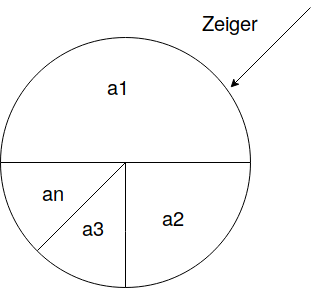
\includegraphics[scale=0.4]{img/roulette_wheel.png}
  \caption{Rouletterad mit Proportinalen Anteil der Individuen anhand ihrere Fitness}
  \label{fig:roulette_wheel}
\end{figure}


introduction to evolutionary comp s80

\iffalse
Problem hier ist das Individuen die am anfang gut sind schnell die ganz epopulation übernehmmen. Das kann dazuführen das eine mögliche bessere lösung durch den Algorithmus im suchraum nicht gefudnen wird. Ein weiteres Problem ist es wenn die Lösungen nahe bei bei einandern liegen gibt es fast keine selections druck mehr herscht. DIes geschied gegen ende der Optimierung und führt zu einem sehr langsamen verlauf gegen ende. 

introduction to evolutionary comp s80
\fi




\item \textbf{Ranking Selektion}, diese Selktion wurde von Backer als Verbesserung der Fitness Proportonal Selection entwickelt \cite{baker1985adaptive}. Dabei werden die Eltern nicht direkt nach ihrer Fitness ausgewählt. Die Fitness dient nur zum einteilen in eine Rangliste. Anhand dieser Rangliste wird dann wieder mit Hilfe des Rouletterades ausgewählt. Dabei gibt es verschiedene Verfahren wie diese Verteilung aussehen kann, einmal ein Lineare Ranking verfahren:
\begin{equation}	
	p_i = \frac{1}{N}(n^- + (n^+ - n^- ) \frac{i-1}{N-1}; i\in{1,...,N} \label{eq:2}
\end{equation}
Wobei $p_i$ die Warscheinlichkeit des i Idividums ist selektiert zu werden. $\frac{n^-}{N}$ ist die Warscheinlichkeit des Schlechtesten Indiviudums selektiert zu werden und  $\frac{n^+}{N}$ ist die Warscheinlichkeit des Besten Individums selektiert zu werden.

oder das expontienelle Ranking:
\begin{equation}
	p_i = \frac{c^{N-i}}{\sum_{j=1}^N c^{N-j}}; i\in{1,...,N} \label{eq:3}
\end{equation}
die Summe $\sum_{j=1}^N c^{N-j}$ normalisiert die Wahrscheilichkeit um sicherzustellen das $\sum_{i=1}^N p_i = 1$
Wobei die Berechnungen \ref{eq:2} und \ref{eq:3} nur den Anteil eines Individums auf dem Rouletterades verändern.

\iffalse
Sie werden nach ihrer Fitness sotiert und einem Rang Rk , k = 1, ...,N wobei N die anteil der individuen einer Population ist. Der beste kandidat erhält den besten Rang wobei der schrlechtestet den Rang N-1 erhält. Die fitness 

 Sie werden in einer Rangliste aufgestellt wobei das beste Individum den Rand y-1 belegt und das schlechteste den Rang 0. Dieses Ranking kann in vielen varianten vorgenommen werden, Linear oder expotenziel umgesetzt werden. 
\fi

\item \textbf{Tunier selektion}, in diesem Verfahren werden züfällig k Induviduen der Population ausgewählt. Diese k Induviuen  tretten wie in einem Tunier gegeneinander an. Der Gewinner ist das Individuum mit dem besten Fittneswert,dieser wird dann auch als Elternteil ausgewählt. Hierbei wird auf den Elternpool verzichtet und direkt ein Kind aus zwei Gewinnern erstellt. Eingesetzt wird dies bei kleineren Populationen mit weniger als 20 Individuen.

\begin{figure}[htb]
  \centering  
  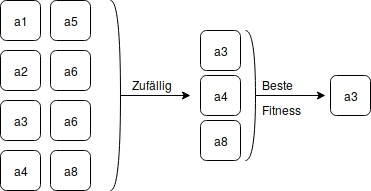
\includegraphics[scale=0.6]{img/Tunier.png}
  \caption{Tunier Selektion mit k = 3 Individuen und dem Gewinner Individuum 3}
  \label{fig:roulette_wheel}
\end{figure}


\end{itemize}


\subsubsection{Vermehrung (eng. Breed)}
Aus dem Elternpool/Paarungspool werden nun Nachkommen(Kinder) geschaffen. Alleine durch die Paarung(eng. Crossover) von qualitativ hochwertigen Individuen wird erwartet, dass die Nachkommen eine bessere Qualität besitzen als die ihrer Eltern. Als zweite Verbesserung wird noch die Mutation einzelner Gene angewendet. Für Crossover und Mutation gibt es verschiedene Ansätze, die in diesem Abschnitt genauer erklärt werden.



\iffalse
Dennoch kann es zu negative man nur die Eigenschaften der Eltern übernimmt kann es sogar dazu kommen das negative eigenschaften mit übernommen werden. Da dies natürlich nicht gewollt ist gibt es eine einfach Verbesserungs möglichkeit. Die Muation, hier wird jedes Gen noch einmal mit einer zufälligen Muation versehen welches ähnliche aber andere Lösungen hervorbringt. Nun gehen wir noch einmal genauer auf Operation Chrossover und Muation ein.

Somit müsste sich die Finttnes der nächsten generation verbessern. Um dies zu ereichen werden die  Gene noch modifiziert, durch corssover oder mutation. Somit wird der suchraum noch einmal vergrößert aber nur in der nähe der für gut empfunden Individuem bzw. dieser Gene.
Um aus den Einzelnen elternpaaren neue Individuen zu generieren wird das Verfahren/algorithmus Crossover verwendet. Bei Crossover kann es nun auch verschiedene möglichkeiten geben.
\fi


\paragraph{Crossover}, nennt man die Operation, bei der die Chromostränge der Kinder Individuen zusammengesetzt werden.
Beim Crossover gibt es mehrer Varianten, die One-Point-Crossover in welchem zufällig ein Punkt im Chromsomenstrang festgelegt wird.
Ab diesem Punkt wird der Chromosomenstrang dann aufgeteilt und anschließend mit dem Crossover des anderne Elternteils wieder zusammen gesetzt. Ein einfaches beispiel ist im Oberenteil der Abbildung \ref{fig:chromoson_crossover} zu sehen.

Eine Abwandlung des one-point-crossover ist das zwei-punkt-crossover oder k-point-crossover. Hier wird der Chromsomenstrang an k punkten aufgeteilt und anschließend wieder zusammengesetzt.
In mittleren Teil der Abbildung \ref{fig:chromoson_crossover}
ist ein k = 2 Crossover zu sehen.

Eine weite Grundlegende Operation beim Crossover ist die Uniformcrossover \cite{Syswerda1989} in welcher es keine Festgelegten punkte gibt. Hier wird für jedes Gen zufällig entschieden aus welchem Elternteil das Gen entnommen wird.
Dies im unteren Teil der Abbildung\ref{fig:chromoson_crossover} noch einmal veranschaulicht.

\begin{figure}[H]
  \centering  
  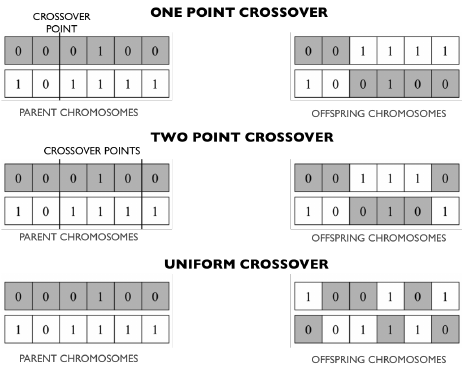
\includegraphics[scale=0.5]{img/Cossover.png}
  \caption{crossover anhand eines einfachen binären Chroms. Das erste zeigt eine 50/50 crossover. Das zweite zeigt eine Zufällige auswahl ders Gens.\cite{Rashid2017} }
  \label{fig:chromoson_crossover}
\end{figure}

Crossover nach dem Paper \cite{Umbarkar2015}.




\paragraph{Mutation},hierbei wird jedes Gen des Individuums zufällig mit einer zufälligen Mutation versehen. Durch diese Mutation wird eine höhere Diversität in die nachfolgende Generation übergeben. Diese Mutation macht es möglich einen größeren Suchraum abzudecken und somit die Werte genauer anzupassen, um so auf die Optimale Lösung zu kommen. 

\begin{figure}[H]
  \centering  
  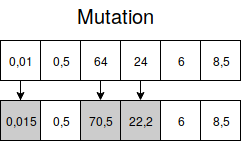
\includegraphics[scale=0.5]{img/mutation.png}
  \caption{Muation eines Genes um höhere vielfältigkeit zubekommen.\cite{Rashid2017} }
  \label{fig:chromoson_mutation}
\end{figure}


\subsubsection{Neue Generation}
Die neue Generation aus Kindern tauscht nun die alte Generation aus. Anschließend folgen die gleichen Schritte so lange bis die gewünschte Abbruchbedingung/ Fitnesswert erreicht ist. Aus dieser letzen Generation kann das beste Individum ausgesucht werden und als beste Lösung weiter verwendet werden. 

\newpage
\subsection{Künstliche Neuronale Netze}

Künstliche Neuronale Netze sind dem natürlichen Vorbild der neuronalen Netze im Gehirn nach empfunden. Beide Netze setzen sich aus einzelnen Neuronen zusammen, welche mit einandern verbunden sind. Wie man in Figure \ref{fig:neural_network} sieht ist jede Schicht ist aus einzelnen Neuronen aufgebaut welche mit den Neuronen der nächsten Schicht verbunden sind, diese Verbindungen repräsentieren die Gewichte, über diese kann einem Netz verschiedene Zusammenhänge von Input und Output antrainiert bzw. angelernt werden.

\begin{figure}[htb]
  \centering  
  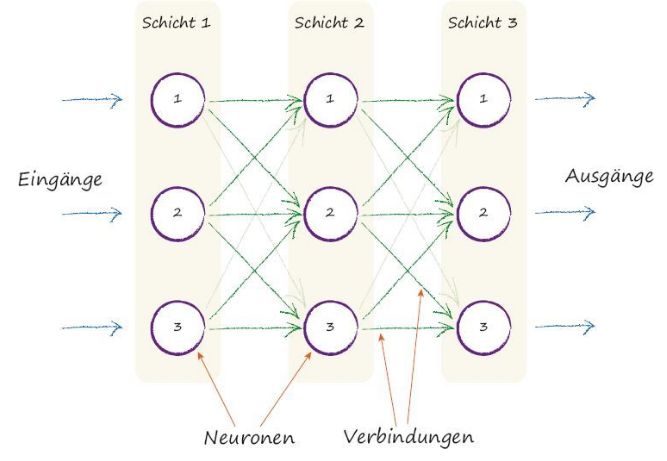
\includegraphics[scale=0.5]{img/S36_Buildyourown.png}
  \caption{Künstliches Neuronales Netz mit drei Schichten je drei Neuronen \cite{Rashid2017} }
  \label{fig:neural_network}
\end{figure}


Im folgenden Kapitel wird zuerst der Aufbau eines Neurons/Perseptron erklärt. Anschließend wird auf den strukturellen Aufbau eines Künstlichen Neuronalen Netzes nähergebracht. Zum Schluss werden noch wichtige Eigenschaften wie die Verlustfunktion und der Gradienten abstieg eingegangen sowie auf die Hyperparameter, welche für die Arbeit essentiell sind.



Grundlagen aus dem buch ArificalNeuroalNetworks s.11 


\subsubsection{Aufbau eines Neurons}



\begin{figure}[htb]
  \centering  
  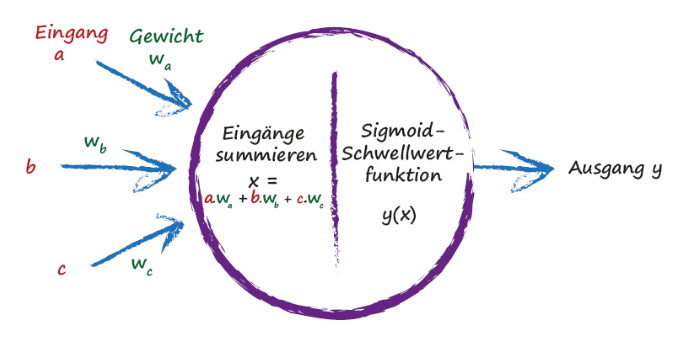
\includegraphics[scale=0.5]{img/S41_Buildyourown.png}
  \caption{Aufbau eines Neurons \cite{Rashid2017}}
  \label{fig:neuron}
\end{figure}

\paragraph{Eingang}
Bei dem Input handelt es sich um einfache xxxFloatwert dieser wird mit den einzelnen Gewichten verrechnet. Ein Neuron hat meist mehrere Eingangsgrößen, welche alle zusammen mit den Gewichten aufsummiert werden. Diese Werte werden zufällig initialisiert und per Training verbessert, somit handelt es sich um einen angelernten Werte, welche durch die Backproagation(Fehlerrückführung) verbessert werden.

\paragraph{Schwellwert aka bias}
Auf dieses Aufsummiertes Ergebniss wird anschließend ein Bias gerechnet, dieser führt zu einem besseren Verhalten beim Trainieren. Bei diesen Werten handelt es sich um angelernte Werte, die per Backpropagation verbessert werden und die Flexibitlität der Netze erhöht.


\paragraph{Aktivierungs Funktion}
Die Aktivierungsfunktion kann man sich als Schwellwert vorstellen, ab wann das Neuron den Input weiter gibt. Es gibt verschiedene Funktionen, um diesen Schwellwert zu definieren. Je nach Aufgabe des Neuronalen Netze werden andere Aktivierungsfunktionen verwendet. Bei Klassifizierungen werden heute meist ReLu-Layer oder ein Weakly-ReLu Layer benutzt, diese verhindern das Vanishing- bzw. Exploding- gradientproblem beim Trainieren.

\paragraph{Ausgang aka Output}
Wenn der Schwellwert überschritten wird, wird am Output durchgeschaltet. Dieser Output kann entweder mit einer nen Schicht Neronen verbundne sein oder direkt als Ausgang gesehen werden. Über welchen man anhand von xxxVariabelenwerten/Kommawerten die 
Von Input nach Output nennt sich ein Single-Forward-Pass. Wie hier beschrieben wird, kann ein Netz verschieden viele Layer besitzen mit verschiedenen Anzahlen von Neuronen.

\subsubsection{Struktureller Aufbau eines Neuronalen Netzes}

Wie kann ich Neuronen zusammenbauen usw.

\paragraph{Input Layer}

\paragraph{Hidden Layer}

\paragraph{Output Layer}

\subsubsection{Verlustfunktion aka lossfunktion}
Die Verlustfunktion stellt ein ausgesuchtes Maß der Diskrepanz zwischen den beobachteten und den vorhergesagten Daten dar. Sie bestimmt die Leistungsfähigkeit des neuronalen Netzes während des Trainings und der Ausführung. Ziel ist es, im laufenden Prozess der Modellanpassung, die Verlustfunktion zu minimieren.

\subsubsection{Optimierer alt Gradientenabstieg}
Um die Fehlerfunktion zu minimieren wird als Werkzeug der Gradienten Abstieg benutzt. Diese ist nur möglich da ein Künstliches Neuronales Netz aus verketteten differenzierbaren Gewichte der Neuronen(Tensoroperationen) aufgebaut ist, die es erlauben duch anwendung der Kettenregel die Gradientenfunktion zu finden, die den aktuellen Parametern des Datenstapels werte des Gradienten zuordnet. Es gibt auch hier verschiedene Ansätze von Optimierern, welche die genauen Regeln wie der Gradient der Verlustfunktion zu Aktualisierund der Parameter verwendet wird hier könnte Beispielweise den RMSProp-Optimierer, der die trägheit des Gradientenabstiegsverfahren berücksichtet.

Seite 83 - Deep Learning chollet


\iffalse
 Im Grunde werden dabei die Gewichte so angepasst, dass ein besseres Ergebnis entsteht und dadurch die Fehlerfunktion verringert wird. Wie das Wort Backpropagation schon sagt, wird von hinten nach vorne verbessert. Es gibt verschiedene Variationen von Gradientenabstiegen, welche verschiedene Vor- und Nachteile haben. Bei dem Trainieren des Netzes wurde der Momentum-Optimizer, welcher aus einem Gradientenabstieg mit Momentum aufgebaut ist.
\fi


\subsubsection{Hyperparameter}
Als Hyperparameter werden, in Bezug auf KNN's, meist die Anfangsbedingungen bezeichnet.
Für diese Hyperparameter gelten keine universellen Werte sondern müssen je nach Daten und Funktion bzw. künstliches Neuroales Netz speziell angepasst und verändert werden. Deshalb gibt es nur einige Regeln und grobe Abschätzungen in welchen grenzen sich diese Hyperparameter befinden. Zu diesen Hyperparameter gehören folgdende:
\begin{itemize}
\item \textbf{Learningrate},blabalaa
\item \textbf{Dropout}
\item \textbf{Lossfunktion}
\item \textbf{Optimizer}
\item \textbf{Model Achitektur}
\end{itemize}

\iffalse
Als Hyperparameter werden, in Bezug auf KNN's, meist die Anfangsbedingungen bezeichnet.
Dabei handelt es sich um die Learnrate (eng. Learningrate), der Abdeckunggrad(eng. Dropout), die Verlustfunktion oder auch der Optimizer. In selten Fällen kann die selbst Modelachitektur als Hyperparameter bezeicht werden. Für diese Hyperparameter gelten keine universellen Werte sondern müssen je nach Daten und Funktion bzw. künstliches Neuroales Netz speziell angepasst und verändert werden. Deshalb gibt es nur einige Regeln und grobe Abschätzungen in welchen grenzen sich diese Hyperparameter befinden. 
\fi


\subsection{Zusammenfassung}





\iffalse
Genetische algorithms ist ein sehr erfolgreiches Oprimiungsverfahren welches es erlaubt auch bei schweren Suchräumen lösungen zu finden. Insbesondere wenn keine gradienten berechnet werden können. In diesem Kapitel wurden die Grundlagen der genetischen Grundlagen zusammengefasst. Sie bassieren auf einer Lösungspopulation, die sich im laufe der iterationen dem Optima annähert. Genetische Operatioren ändern die Lösungen. Cross-overoperatoren kobinieren genome zweier Lösungen. Die Mutation fügt den Lösungen Zufälligkeiten hinzu und sollte somit jenden Ort im Lösungsraum erreichen. Der Genotyp oder Das Chromosom einer Lösing wird auf einen Phänotyp, die reale Lösung, abgebildetet, bevor es mit einer Fintessfunktion ausgewertet werden kann. Diese Fittnesfunktion muss sehr sorgfällig ausgearbeitet werden, da sie einen entscheidenden einfluss auf die Suche hat. Die Lösungen mit der höchsten fittnes sind folglich die Eltern der nächsten generation. Sobald eine Generation eine bestimmte Fintess ereicht sprich genug Optimiert wurde ist die beste Lösung gefunden. Somit wurde ein Algorithmus vorgestellt welcher auf ein breites Spektrum von Probkemen anwendbar ist.

Genectic - algorhmen - essential s.19 
\fi

\cleardoublepage

\chapter{Stand der Technik und Forschung}
\section{Stand der Forschung und Technik}
Durch die gestiegene Rechenleistung der heutigen Computer ist auch die anwendungshäufigkeit deutlich gestiegen. 
Es werden nicht nur neue Ansätze von großen Unternehmmen wie Google Deepmind entwickelt. Sondern auch kleiner anwendungen die nicht nur im IT-Bereich ihre anwendungen finden.

\subsection{Deep Mind}
Den größten Fortschitt der letzen Jahre verzeichnete Googles Deepmind. Google setzt dabie auch auf einen Populations bassierenden Algorithmus welcher auf den Genetischen Algorithmen aufbaut. Zum selbst Algortihmus später mehr. Goolge nutz ihre PopulationBasedTraining vorallem im Bereich der Künstlichen Inteligzenz. So konnten sie bei verschiedene Knns wie AlphaGo(Go)\cite{alphago} und AlphaStar(Starcraft2)\cite{alphastar} deutliche verbesserungen durch das PBT erreichen. Google verwendet PBT nicht nur für Brett- bzw. Computer-spiele sodnern auch für Anwendungen im Bereich des autonomen fahrens in zusammenarbeit mit der Google-Tochter Waymo. 

\subsection{PopulationBasedTraining}
PBT ist eine weiter entwicklung der klassischen Grid- und Randomsearch und wird von den Genetischen Grundlagen stark beinflusst. Dies ist zusehen daran das PBT auch eine Population verwendet, auch werden hier die übernahmme des Fitesten und Muationen verwendet. Zudem ist das Training Asynchron und Parallel möglich.
Desweitern wurde ein online anpassung der Hyperparameter wärend des Trainings implementiert. Durch dieses Feature, wird viel Rechenleistung eingespaart bzw. das berechnen der Hyperparameter stark beschleunigt. \cite{pbt}


\iffalse
Sie verwenden Algorithem die dem GA Sehr ähnlich(weiter entwickelt) ist und zwar das Population bassierende Training (eng. Poulation Based Training short PBT). Sie benutzen PBT auch zum anpassen von Hyperparametern speziel für ihre Reinforcment Learning Models. Deep Minds Variante des GA ist sehr viel komplexer. 
Sie haben ein Online-Learn verfahren in welchem sie die Hyperparameter während des Trainings anpassen können, dies ist durch einen einen Server auf dem die daten gespeichert sind möglich. Dieser gibt ihnen auch die möglichkeit Asynchron und Parallel zu arbeiten. Im Durschnitt kontne sie ihre Ergebnisse noch einmal um bis zu 5 Prozent verbessern. 
\fi

\subsection{Software Testing with Ga}
Die Softwarebewertung spielt eine entscheidende Rolle im Lebenszyklus eines Software-Produktionssystems. Die Erzeugung geeigneter Daten zum Testen des Verhaltens der Software ist Gegenstand vieler Forschungen im Software-Engineering.  In diesem Beitrag wird die Qualitätskontrolle mit Kriterien zur Abdeckung von Anwendungspfaden betrachtet und ein neues Verfahren auf der Grundlage eines genetischen Algorithmus zur Erzeugung optimaler Testdaten vorgeschlagen. 
\cite{Keshavarz}


\subsection{Travelling Salesman Problem}
Einer der bekanntesten anwendungen ist das Travelling Salesman Problem, in welchem die kürzeste Route für einen Postboten berechnet werden soll. Doch je mehr Briefe der Postbote austragen soll umso mehr Variablen gibt es, sprich es wird wesentlich schwerer für ein fest geschrieben (eng. Hardcoded) Algorithmus den kürzesten weg zu finden. Für den Ga ist dies kein Problem da mit der richtigen Fitnessfunktion eine einfacher Rückgabewert der Funktion zu bekommen ist. Dementsprechend kann die Route einfach optimiert werden.

\subsection{Temperatur Schätzungen}
Es gibt auch Forschungen zur berechnung von Temperaturverläufen der Erde \cite{Stanislawska1}. Vom gleichen Author gibt es auch eine abschätzungen von Wäreme flusses zwischen Athmosphäre und Meereies in Polarregeionen \cite{Stanislawska2}. All diese Berechnungen wurden mithilfe von Genetischen Algorithmen ausgerechnet. In dem die Aufzeichnungen der Temperaturverläufe als Trainingsdaten verwendet werden konnten Lösungen gefunden werden, welche den rellen daten sehr nahe kommen.

\subsection{Generativ Design}
Heute gibt es in viele Computer-aided design(CAD) Programme in welchen es implementierungen von Generativen Design Werkzeugen gibt. In dennen über Iterationen neue mögliche Designs berechnet werden deis passiert auch auf Basis der Genetischen Evolution. Sie bauen nicht auf den Genetischen Algorithmen auf sind aber nahe verwante und sollten nicht unterschätzt werden. 
Mit ihnen ist es möglich Bionische Stukturen für addetive Vertigung zu designen. Und sie speziell auf die Anwendung anpassen. So kann aus einem einfachen Frästeil ein wesentlich Leichtes und Material spaarenderes Model entwickelt werden.

\noindent%
\begin{figure}[H]
  \centering  
  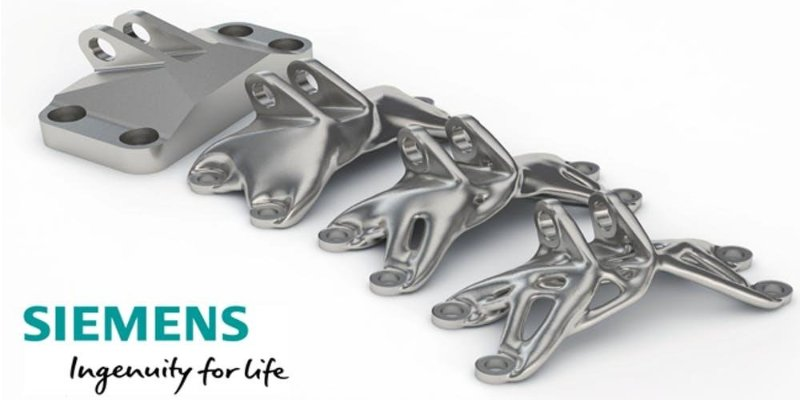
\includegraphics[scale=0.3]{img/Additive.png}
  \caption{Additives Design über mehrer Iterationen}
  \label{fig:Ablauf_kurz}
\end{figure}

\paragraph{NASA - Antenne}
DIe Nasa hat 2006 eine Weltraumantenne mit hilfe evolutionären Algorithmen entwickelt. Die Entwicklung der Antenne von hand ist sehr zeitaufwändig und arbeitsintehnsiv, zusätzlich braucht man großes wissen in der entsprächenden Domain. Deshalb nutzen die Forscher einen Populations bezogenen Suchansatz, um Umgebungsstrukturen und  elektromagnetischer mit einzubeziehen. Die entwickelte Antenne wurde produziert und auch auf Space Technology 5 mission genutzt.
\cite{AutomatedAntenna}
\noindent%
\begin{figure}[H]
  \centering  
  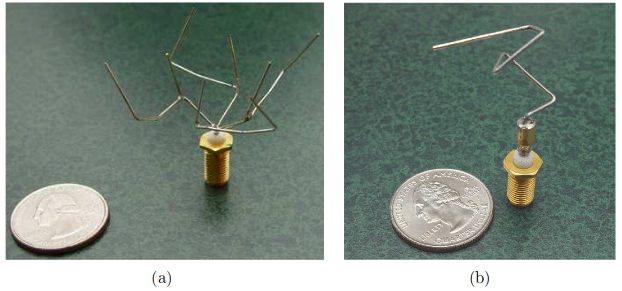
\includegraphics[scale=0.5]{img/nasa-antenne.png}
  \caption{Foto der Prototypen. Für die Antennen wurden verschiedene Anforderungen als Grundlage gegeben. \cite{AutomatedAntenna}}
  \label{fig:Ablauf_kurz}
\end{figure}


\subsection{GLEAM}
General Learning Evolutionary Algorthm and Method ist eine vom Kit entwickelte Methode um Aktionsketen zu berechnen. Dazu gehörtz zum beispiel das Aufeinandern abstimmen der Maschinen in einem Maschinenpark um so genannte totzeiten der Maschinen zu verringern also die gesamt auslastung zu erhöhen.

Mit GLEAM wurde auch versucht die Stuerung von 6-Achsigen Robotorarmen zu verbessern. Es konnte gezeigt werden das die Steuerung mit Gleam funktioniert, dies wurde aber leider nie der neue Industie Standart. Es wird immer noch mit der klasschischen xxxSteuerungxxx  gearbeitet. 


\subsection{Reainforcment learning with GA}
Reinforcment learning ist möglichweise einer der größten Anwendungsgebiete der GA. Hierbei werden Neuronale Netze nicht mit hilfe von Gradienstieg training, wie im Gundlagen Kapitel besprochen. Sondern mit hilfe von Genetischen Algorithmen. Dabei wird das Neuronale Netz nicht 




\subsection{Zusammenfassung}
\cleardoublepage

\chapter{Konzept}
\section{Konzept}
\subsection{Anforderungsanalyse}



\subsection{Genetischer Algorithmus}
\subsubsection{Eltern auswahl} 
Ranking Selction mit 50 übernahme als Eltern.
Zusätzlich werden die besten 4 Eltern ganz übernommen. das die Generationen sich nicht zu sehr ähnlichsind wird hoh mutation bei den Kindern. Zusätzlich werden bei jeder neuen Generation immer ein paar neu und damit zufällige Individuen hinzu gefügt. 

Best 50 prozent,heißt aus der oberen hälfte der alten Generation werden alle Induviduen dem Elternpool hinzugefügt. Aus welchen dann zufällig die einzelnen Elternteile ausgewählt werden. Es mssen natürlich nicht immer 50 prozent sein, es kann sich auch um einen anderen Prozentsatz handeln.


\subsection{Zusammenfassung}
\cleardoublepage

\chapter{Implementierung}
In diesem Kapitel werden die Implementierungen dieser Arbeit erläutert. Zuerst wird der Systemaufbau erklärt und alle verwendeten Module ausführlich beschrieben. Anschließend wird auf die verwendete Hardware eingegangen. Im Folgenden werden die implementierten Methoden des GA und der Zufallssuche genauer betrachtet, indem die exakten Methoden und künstlichen neuronalen Netze erklärt werden. Zum Schluss wird auf die implementierten Evaluationen und Auswertungen eingegangen. 

\section{Systemaufbau}
Das Gesamtsystem wird mit Python als Programmiersprache umgesetzt. Für die Implementierung werden zusätzliche Python Pakete verwendet. 
Für das Erstellen und Trainieren der künstlichen neuronalen Netze wird auf Tensorflow zurückgegriffen. Tensorflow ist eine End-to-End-Open-Source Plattform für maschinelles Lernen (ML). Zudem bietet Tensorflow ein umfassendes und flexibles Ökosystem aus Werkzeugen und Bibliotheken für ML-Anwendungen. Darüber hinaus hat Tensorflow eine starke Community, welche vorallem im ML-Bereich viele Open-Source-Projekte entwickelt und veröffentlicht.
Für die Zufallssuche wird SkLearn verwendet. Bei SkLearn handelt es sich um ein simples und effizientes Werkzeug zur prädiktiven Datenanalyse. Dies beinhaltet Funktionen wie:  Klassifikation, Regression, Clustering, Support Vektor Maschine. Mit Hilfe von SkLearn werden die bewertungsmatrixen zum Auswerten der Algorithmen umgesetzt.
Zum Darstellen von Diagrammen wird Seaborn und Matplotlib verwendet.
Der Genetische Algorithmus wurde eigenständig implementiert. Für diesen wurden nur die Pakete Numpy und Pandas verwendet. Numpy ist ein Paket für Multi-Dimensionen Arrays und bietet eine große Anzahl an mathematischen Funktionen. Pandas ist wie Numpy für Arrays und Datenframes zuständig. Im Detail ist Pandas für Datenstrukturen und Manipulation solcher Datenarrays entwickelt worden.
Da die Rechenzeit ein entscheidender Faktor der Optimierung darstellt, wird das Paket Multiprocessing verwendet. Dies führt vor allem bei Multi-Core-Servern zu schnelleren Berechnungen. Das Gesamtsystem wurde für CPU entwickelt. Darüber hinaus ist der Genetischen Algorithmus als GPU (engl. graphics processing unit) optimierte Implementierung vorhanden. Dies beschleunigt die Berechnungen von großen KNNs deutlich. 
All diese Einstellungen können per Argumente an das Python Skript übergeben werden. Somit ist es einfach möglich andere Berechnungen durchzuführen, auch solche, die in dieser Arbeit nicht besprochen werden. Eine ausführliche Auflistung aller verwendeten Pakete ist in Abbildung \ref{fig:Python_pakete} zu sehen. 

\begin{figure}[H]
  \centering  
  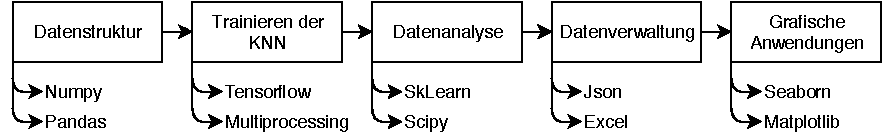
\includegraphics[scale=1]{img/Python_pakete.pdf}
  \caption{Datenfluss und verwendete Python Pakete, die zur Umsetzung der Arbeit verwendet wurden}
  \label{fig:Python_pakete}
\end{figure}

\subsection{Hardware}
Um die Optimierungen durchzuführen stehen drei Hardwaremöglichkeiten zur Auswahl. Dazu gehört ein Server mit i5-5550 Prozessoren mit 40 Kernen ohne GPU, ein Server mit einer Grafikkarte (Gtx1080Ti) um die Berechnungen durchzuführen und eine Server mit einem i7-7700 Prozessor mit 8 Kernen ohne GPU. Diese sind tabellarisch in Tabelle \ref{tab:Server} aufgeführt. Im späteren Kapitel \ref{sec:Evaluierung} wird auf die Benchmarks der Hardware eingegangen.

\begin{table}[htb]
\centering
\caption{Zur Verfügung stehende Hardware} \label{tab:Server}
\begin{tabular}{lccc}\toprule
\textbf{Hardwarekomponenten}	&\textbf{Server 1} &\textbf{Server 2} &\textbf{Server 3}	\\\midrule
Prozessor		& E5-2630   & i7-7700	& i7-7700 \\
Logische Kerne 	& 40        & 8     	& 8 	\\
Arbeitsspeicher	& 256 GB    & 8 GB	    & 32 GB	\\
Grafikkarte		& -	        & -	        & GTX 1080 Ti (11 GB)	\\\bottomrule
\end{tabular}
\end{table}


\subsection{Datensatz}
Um die künstlichen neuronalen Netze zu trainieren wurden Bilddaten als Daten-Grundlage ausgewählt. Bei den verwendeten Datensätzen handelt es sich um gängige Datensätze, die oft zum Vergleichen von Klassifikationsergebnissen von KNN genutzt werden. Folgende Datensätze wurden ausgewählt: Mnist Faschion, Mnist Digits und Cifar10. Diese drei Datensätze werden benutzt, da sie sich sehr ähnlich sind. Alle drei besitzen eine gleichmäßige Verteilung der Daten in Bezug auf die Klassen. Die Datensätze besitzen jeweils 10 Klassen. Die Besonderheit der Datensätze liegt auf ihrer guten Vergleichbarkeit. Die einzigen Unterschiede sind die Klassen und Bildformate. Alle verwendeten Datensätze werden wie folgt aufgeteilt: 65\% Trainingsdaten, 20\% Validierungsdaten, 15\% Testdaten. Somit wird das Overfitten der Netze verhindert, da die Daten klar getrennt werden. Nachfolgend werden die Datensätze genauer beschrieben.

\paragraph{Mnist Fashion Datensatz}
Zur Evaluierung der Methoden des Genetischen Algorithmus wurde der "`Mnist Fashion"' Datensatz benutzt. Dieser Datensatz enthält 10 Klassen für verschieden Kleidungsstücke. Er beinhaltet die Klassen: T-shirt/Top, Trouser, Pullover, Dress, Coat, Sandal, Shirt, Sneaker, Bag, Ankle Boot. Der Mnist Fashion Datensatz besteht aus 70.000 Schwarz-weiß Bildern mit je 28x28 Pixeln. Ein Beispiel aus dem Datensatz ist in Abbildung \ref{fig:dataset_example} auf der linken Seite zusehen. 

\paragraph{Mnist Digits Datensatz}
Zum Evaluieren der Optimierung des Fully Conneceted Netzes wird der "`Mnist Digits"' Datensatz benutzt. Dieser besteht aus handgeschrieben Ziffern zwischen 0 und 9. Der Mnist Digits Datensatz besteht aus 70.000 Schwarz-weiß Bildern mit je 28x28  Pixeln. Ein Beispiel des Mnist Digits Datensatze ist in der Mitte der Abbildung \ref{fig:dataset_example} zusehen. Um die Evaluation der Optimierung nicht nur mit einem Datensatz durchzuführen, wird ein dritter Datensatz verwendet.

\paragraph{Cifar 10 Datensatz}
Hierbei handelt es sich um den CIFAR 10 Datensatz. Er besitzt die Klassen: Flugzeug, Auto, Vogel, Katze, Reh, Hund, Pferd, Schiff und LKW. Der Datensatz ist aus 60.000 farbigen Bildern (RGB) mit je 32x32 Pixel aufgebaut. Ein Beispiel ist auf der rechten Seite der Abbildung \ref{fig:dataset_example} zusehen. 

\begin{figure}[H]
  \centering  
  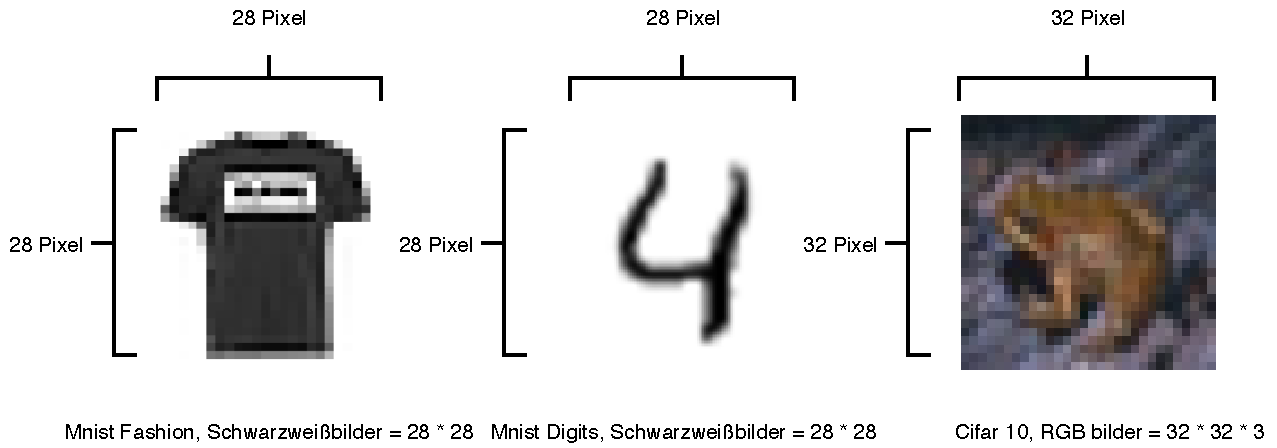
\includegraphics[scale=0.7]{img/dataset_example.pdf}
  \caption{Beispiele aus den verwendeten Datensätze}
  \label{fig:dataset_example}
\end{figure}

\section{Genetischer Algorithmus} \label{ssec:implementierung}
Die Implementierung des Genetischen Algorithmus entspricht den 5 Schritten des Genetischen Algorithmus, das Konzept wurde in Kapitel \ref{ssec:GA} beschrieben. In den folgenden Unterkapitel werden die implementierten Methoden im Detail besprochen. Zusätzlich wird auf speziellen Umsetzungen und Eigenschaften eingegangen. Da es zu den meisten Methoden in der Literatur wenig Informationen zu ihren Auswirkungen auf das Endergebnis gibt, wird ein Experiment zur Bestimmung der zielführenden Methoden durchgeführt. Für dieses Experiment wurde eine Optimierung der Hyperparameter durchgeführt. Als Netz wird ein Fully-Connected Netz mit einem Layer und 128 Neuronen verwendet, die Größe des Netzes wird im Abschnitt \ref{tab:fully_small} ausführlich beschrieben. Es wurde diese Größe gewählt, da die spätere Evaluation mit der gleichen Größe an Netz durchgeführt wird. Als Datengrundlage wurde der Mnist Fashion Datensatz verwendet, linke Seite der Abbildung \ref{fig:dataset_example}. Die Methoden mit den die besten Ergebnisse gefunden wurden, werden zur Evaluierung des Genetischen Algorithmus eingesetzt. Das Wissen zu den Grundlagen der Methoden des Genetischen Algorithmus wird für dieses Kapitel als voraussetzt angenommen und kann im Grundlagenkapitel \ref{Genetische_Algorithmen} nachgelesen werden.

\newpage

\subsection{Initialisierung der Anfangspopulation} \label{implementierung_init}
Die Größe der Anfangspopulation kann beliebig bestimmt werden. Im späteren Evaluationsabschnitt \ref{sec:Evaluierung} wird die genauen Größe definiert, da diese im direkten Zusammenhang mit der Laufzeit steht. Der Suchraum in dem die Hyperparameter zufällig initialisiert werden, ist in Tabelle \ref{tab:Rahmen} zusehen. Die Grenzen des Suchraums wurde mithilfe der Literatur und des beschriebenen Experiments bestimmt. Die Initialisierung im Suchraum ist zufällig mit einer gleichmäßigen Verteilung umgesetzt. Diese ist als Formel in Eq. \ref{eq:10} abgebildet.

\begin{equation}
	p(x) = \frac{1}{b - a}  \label{eq:10}
\end{equation}
a und b bilden die Intervallgrenzen.

\begin{table}[htb]
\centering
\caption{Suchraum des Genetischen Algorithmus}\label{tab:Rahmen}
\begin{tabular}{lccc}\toprule
\textbf{Hyperparameter}	&\textbf{Minimum}   &\textbf{Maximum}	\\\midrule
Prozessor		        & 0.000005          & 0.1 \\
Logische Kerne 	        & 0.05          	& 0.5 \\
Arbeitsspeicher     	& 10                & 80	\\
Grafikkarte		        & 0	                & 7	\\\bottomrule
\end{tabular}
\end{table}
Hierbei steht jede ganze Zahl beim Optimierer für einen eigenen Optimierer. Hierbei entspricht: 0 = adam, 1 = SGD, 2 = RMSprop, 3 = Adagrad, 4 = adadelta, 5 = adammax, 6 = nadam, 7 = ftrl


\subsection{Fitnessfunktion}\label{implementierung_Fitnessfunktion}
Die Fitnessfunktion beinhaltet den rechenaufwendigsten Teil der Arbeit. In dieser werden die KNNs berechnet. Dazu werden die Gene (Hyperparameter) als Input verwendet. Anschließend werden die Daten geladen, das Netz trainiert und anschließend evaluiert. Der Rückgabewert ist die Klassifizierungsgenauigkeit, die dem Fitnesswert entspricht. Die Fitnessfunktion ist in Abbildung \ref{fig:Fitnessfunktion} als Whitebox dargestellt. Die Fintessfunktion wird für unterschiedliche KNN erstellt. Diese Netze sind im Kapitel \ref{sec:Evaluierung} beschreiben.

\noindent%
\begin{figure}[H]
  \centering  
  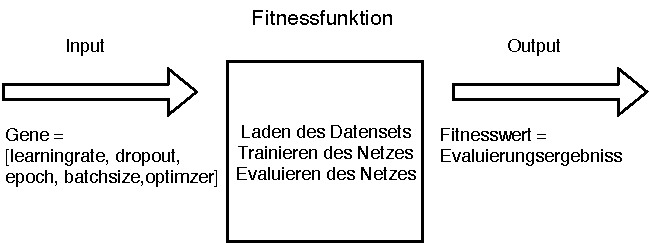
\includegraphics[scale=1]{img/Fitnessfunction.pdf}
  \caption{Beispielhafte Whitebox der Fitnessfunktion mit Genen als Input und Klassifikationsgenauigkeit als Output}
  \label{fig:Fitnessfunktion}
\end{figure}  


\subsection{Selektion der Eltern} \label{implementierung_Selektion_Eltern}
Aus dem Experiment hat sich gezeigt, dass bei der Selektion der Eltern die Fitness proportional Selektion(FPS) die besseren Ergebnisse im Vergleich zu der Ranking Selektion liefert. Aus diesem Grund wird die FPS bei der Evaluation des Genetischen Algorithmus verwendet.

\subsubsection{Vermehrung} \label{implementierung_vermehrung}
Für das \textbf{Crossover} wurde Two-Point Crossover und Uniform-Crossover implementiert. Für die \textbf{Mutation} wurde die Gauss-Mutation mit der Gaussdichteverteilung, mit Sigma gleich 0.1 (Eq. \ref{eq:11}) und eine Mutation mit gleichmäßiger Verteilung (Eq. \ref{eq:10}) implementiert. Für die spätere Evaluation der Optimierung mit dem GA wurde Two-Point Crossover und die Gauss-Mutation ausgewählt, da sie in den Experimenten die zielführendsten Ergebnisse lieferten.

\begin{equation}
	p(x) = \frac{1}{\sqrt{ 2 \pi \sigma^2 }} e^{ - \frac{ (x - \mu)^2 } {2 \sigma^2} } \label{eq:11}
\end{equation} 

\newpage

\subsection{Neue Generation}
Die Population der neuen Generation wird mit den genannten Methoden ausgewählt. Diese sind in Abbildung \ref{fig:Ga_Methoden} noch einmal dargestellt. Die Experimente zeigten, dass die Optimierungsergebnisse sich steigern lassen, wenn die besten zwei Individuen der alten Generation, ohne Mutation und Crossover, in die nächste Generation übergeben werden. Dies kann für beliebig viele Generationen durchgeführt werden oder bis zum Erreichen einer Abbruchbedingung.

\noindent%
\begin{figure}[H]
  \centering  
  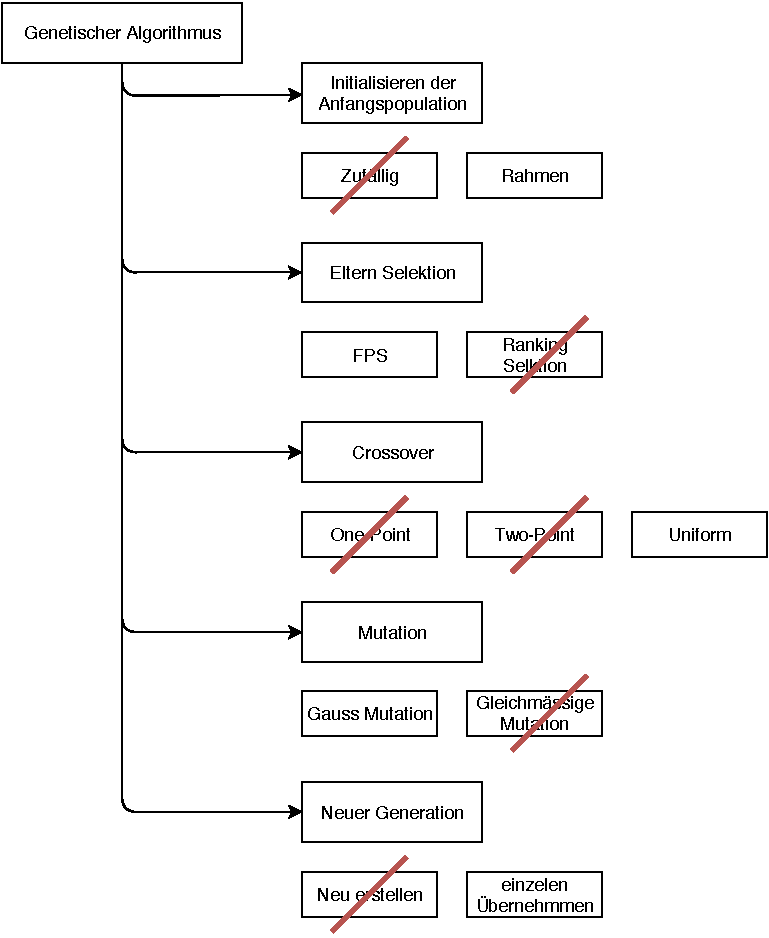
\includegraphics[scale=0.9]{img/Ga_Methoden.pdf}
  \caption{Implementierte und verwendete Methoden des Genetischen Algorithmus}
  \label{fig:Ga_Methoden}
\end{figure}

\section{Zufallssuche}
Die Zufallssuche wird mit Hilfe der Python Bibliothek SkLearn umgesetzt. Die implementierte Zufallssuche ist, wie im Grundlagenkapitel \ref{Zufalls_Suche} beschrieben, aufgebaut. Für den Suchraum der Zufallssuche gelten die gleichen Rahmenbedingungen wie für den Genetischen Algorithmus. Im Vergleich zum GA wird der Suchraum bei der Zufallssuche in ein Raster aufgeteilt. Dieses Raster ist in Tabelle \ref{tab:Raster} zusehen.


\begin{table}[htb]
\caption{Suchraum der Zufallssuche} \label{tab:Raster}
\begin{tabular}{lccclllll}\toprule
\textbf{Hyperparameter} &\textbf{Min}   &   &   &   &   &  &   &\textbf{Max}	\\\midrule
Lernrate       & 0.00005 & 0.0001 & 0.0005 & 0.001 & 0.005 & 0.01 & 0.05 & 0.1  \\
Dropout        & 0.05    & 0.1    & 0.2    & 0.3   & 0.4   & 0.5  & 0.6  & 0.7  \\
Epochen        & 10      & 20     & 30     & 40    & 50    & 60   & 70   & 80   \\
Batchsize      & 8       & 16     & 32     & 40    & 48    & 56   & 64   & 72   \\
Optimizer      & 0       & 1      & 2      & 3     & 4     & 5    & 6    & 7    \\\bottomrule
\end{tabular}
\end{table}

Jede ganze Zahl des Optimizer steht für einen eigenen Optimierer. Hierbei entspricht 0 = adam, 1 = SGD, 2 = RMSprop, 3 = Adagrad, 4 = adadelta, 5 = adammax, 6 = nadam, 7 = ftrl.

\section{Evaluierung} 
\label{sec:Evaluierung}
Zur Evaluierung wird die Berechnungszeit der beiden Algorithmen gleichgesetzt. Da das Trainieren der KNN 95\% der Berechnungszeit der Algorithmen ausmacht, wird die Berechnungszeit über die Anzahl der Trainingsvorgänge begrenzt. Durch Versuche ergab sich die Evaluierung von 50 und 250 Iterationen als zielführend. Eine weitere Verdopplung der Iterationen von 250 auf 500, zeigte bei den Versuchen keine Verbesserung der Ergebnisse. Trotz des doppelten Rechenaufwandes. Aus diesem Grund ist die Berechnung von 500 Iterationen nicht umgesetzt worden. Für die Zufallssuche ergibt sich somit 50 und 250 Iterationen. Für den Genetischen Algorithmus ergibt sich für 50 Iterationen eine Populationsgröße von 25 Individuen mit 2 Generationen. Für 250 Iterationen wird im GA eine Populationsgröße von 50 Individuen und 5 Generationen gewählt. Um aussagekräftige Ergebnisse zu erhalten wurden zwei KNNs implementiert:


\subsection{Hyperparameter Optimierung - Fully Connected Network}
Es wird ein Fully Connected Network zur Klassifizierung von handgeschriebenen Ziffern implementiert. Darüber hinaus werden zwei verschiedene Größen des künstlichen neuronalen Netzes implementiert, um mögliche Unterschiede der Modellgröße auf die Optimierung zu erkennen. Für das Fully-Connected-Network wurden diese Größen von KNNs implementiert:
\begin{itemize}
\item \textbf{kleines KNN} mit einem Layer und 128 Neuronen. Die exakte Modell-Architektur ist in der nachfolgenden Auflistung zusehen. Die 28x28 Pixel der Eingangsdaten werden zu 784 Pixel mit nur einer Dimension flachgedrückt (engl. flatted). Anschließend kommt die Versteckteschicht (engl. hidden Layer) mit 128 Neuronen und einer  Dropoutschicht, die für jedes Neuron durchgeführt wird. Abschließend kommt die Ausgangsschicht mit 10 Klassen, wodurch sich 10 Neuronen in der Ausgangsschicht ergeben. Dies entspricht einer Anzahl von 101.770 trainierbaren Parametern. Somit ist dieses Netz im Vergleich zu State-of-the-Art Netzen relativ klein. Diese Netz ist beispielhaft als Figur \ref{fig:mlp_128} und als Auflistung in der Liste \ref{auflistung_fully_klein} zusehen.

\noindent%
\begin{figure}[H]
  \centering  
  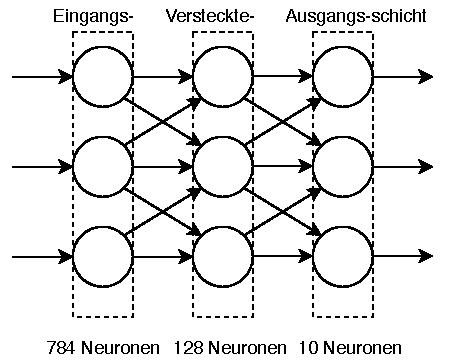
\includegraphics[scale=0.9]{img/mlp_128.pdf}
  \caption{Beispielhafte Darstellung des kleinen KNNs}
  \label{fig:mlp_128}
\end{figure}


Beispielhaft wird die Trainingsdauer des kleinen Netzes für 10 und 80 Epochen evaluiert. Bei 10 Epochen dauerte der Trainingsvorgang 34 Sekunden und für 80 Epochen 252 Sekunden. Diese Werte wurden auf einem Intel i7-7700 3,6 GHz erreicht.
\newpage
{\small
\begin{lstlisting}[language=C,caption=Exakte Modell-Architektur des kleinen Fully-Conneted-Networks,label=auflistung_fully_klein]
_______________________________________________________________
Layer (type)                 Output Shape              Param #
===============================================================
flatten (Flatten)            (None, 784)               0
_______________________________________________________________
dense (Dense)                (None, 128)               100480
_______________________________________________________________
dropout (Dropout)            (None, 128)               0
_______________________________________________________________
dense_1 (Dense)              (None, 10)                1290
===============================================================
Total params: 101,770
_______________________________________________________________
\end{lstlisting}
}

\item \textbf{großes KNN} mit zwei Layer je 128 Neuronen. Die exakte Modell-Architektur ist in der nachfolgenden Auflistung zusehen. Die 28x28 Pixel der Inputdaten werden zu 784 Pixel mit nur einer Dimension flachgedrückt. Anschließend kommt die erste Versteckteschicht mit 128 Neuronen und einer Dropoutschicht, die für jedes Neuron durchgeführt wird. Nun kommt erneut eine Versteckteschicht und Dropout mit 128 Neuronen. Abschließend kommt die Ausgangsschicht mit 10 Klassen, wodurch sich 10 Neuronen in der Ausgangsschicht ergeben. Dies entspricht einer Anzahl von 134.794 trainierbaren Parametern. Somit ist das Netz im Vergleich zu State-of-the-Art Netzen relativ klein. Diese Netz ist beispielhaft als Figur \ref{fig:mlp_2x128} und als Auflistung in der Liste \ref{auflistung_fully_groß} zusehen.

\noindent%
\begin{figure}[H]
  \centering  
  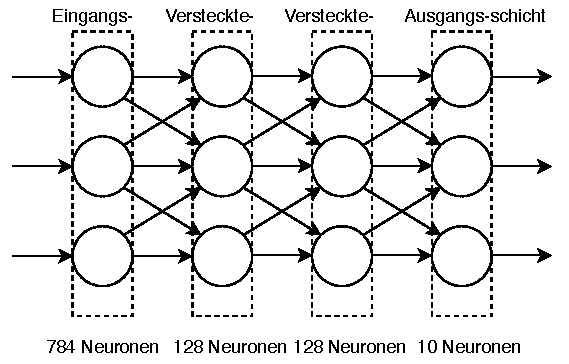
\includegraphics[scale=0.9]{img/mlp_2x128.pdf}
  \caption{Beispielhafte Darstellung des großen KNNs}
  \label{fig:mlp_2x128}
\end{figure}

Beispielhaft wird die Trainingsdauer des großen Netzes für 10 Epochen und 80 Epochen evaluiert. Bei 10 Epochen dauerte der Trainingsvorgang 44 Sekunden und für 80 Epochen 339 Sekunden. Diese Werte wurden auf einem Intel i7-7700 3,6 GHz erreicht. 

{\small
\begin{lstlisting}[language=C,caption=Exakte Modell-Architektur des großen Fully-Conneted-Networks,label=auflistung_fully_groß]
_______________________________________________________________
Layer (type)                 Output Shape              Param #
===============================================================
flatten (Flatten)            (None, 784)               0
_______________________________________________________________
dense (Dense)                (None, 128)               100480
_______________________________________________________________
dropout (Dropout)            (None, 128)               0
_______________________________________________________________
dense_1 (Dense)              (None, 128)               16512
_______________________________________________________________
dropout_1 (Dropout)          (None, 128)               0
_______________________________________________________________
dense_2 (Dense)              (None, 128)               16512
_______________________________________________________________
dropout_2 (Dropout)          (None, 128)               0
_______________________________________________________________
dense_3 (Dense)              (None, 10)                1290
===============================================================
Total params: 134,794
_______________________________________________________________
\end{lstlisting}
}


\end{itemize}

\subsection{Hyperparameter Optimierung - Convolutional Neural Network}
Es wurde ein faltendes neuronales Netz (engl. Convolutional Neural Network - CNN) zur Klassifizierung von kleinen RGB Bildern aus dem Cifar10 Datensatz implementiert. Die exakte Modell-Architekturen ist in der nachfolgenden Auflistung zusehen.
Beim CNN werden die Pixel nicht flachgedrückt, sondern können als Matrix geladen werden. Anschließend kommen verschiedene Kombinationen aus Convolutionalschicht, Activationschicht, Dropoutschicht und Maxpoolingschicht. Diese Schichten besitzen deutlich mehr Parameter. Dieses CNN besitzt 1.250.858 trainierbare Parameter und besitzt damit fast 10 Fach so viele trainierbaren Parametern wie die FCN.

Beispielhaft wird die Trainingsdauer des CNN-Netzes für 10 Epochen und 80 Epochen evaluiert. Bei 10 dauerte der Trainingsvorgang 15 Minuten und für 80 Epochen 125 Minuten. Diese Werte wurden auf einem Intel i7-7700 3,6 GHz erreicht. 

{\small
\begin{lstlisting}[language=C,caption=Exakte Modell-Architektur des Convolutional Neural Network ,label=auflistung_cnn]
_______________________________________________________________
Layer (type)                 Output Shape              Param #
===============================================================
conv2d (Conv2D)              (None, 32, 32, 32)        896
_______________________________________________________________
activation (Activation)      (None, 32, 32, 32)        0
_______________________________________________________________
conv2d_1 (Conv2D)            (None, 30, 30, 32)        9248
_______________________________________________________________
activation_1 (Activation)    (None, 30, 30, 32)        0
_______________________________________________________________
max_pooling2d (MaxPooling2D) (None, 15, 15, 32)        0
_______________________________________________________________
dropout_1 (Dropout)          (None, 15, 15, 32)        0
_______________________________________________________________
conv2d_2 (Conv2D)            (None, 15, 15, 64)        18496
_______________________________________________________________
activation_2 (Activation)    (None, 15, 15, 64)        0
_______________________________________________________________
conv2d_3 (Conv2D)            (None, 13, 13, 64)        36928
_______________________________________________________________
activation_3 (Activation)    (None, 13, 13, 64)        0
_______________________________________________________________
max_pooling2d_1 (MaxPooling2 (None, 6, 6, 64)          0
_______________________________________________________________
dropout_2 (Dropout)          (None, 6, 6, 64)          0
_______________________________________________________________
flatten_1 (Flatten)          (None, 2304)              0
_______________________________________________________________
dense_2 (Dense)              (None, 512)               1180160
_______________________________________________________________
activation_4 (Activation)    (None, 512)               0
_______________________________________________________________
dropout_3 (Dropout)          (None, 512)               0
_______________________________________________________________
dense_3 (Dense)              (None, 10)                5130
_______________________________________________________________
activation_5 (Activation)    (None, 10)                0
===============================================================
Total params: 1,250,858
_______________________________________________________________
\end{lstlisting}
}

\subsection{Hyperparameter Optimierung - kleiner Datensatz}
Bei der Optimierung mit kleinen Datensätzen wird geprüft, ob sich andere Ergebnisse beim Optimieren der Hyperparameter mit kleinerem Datensatz zeigen. Dazu werden die gleichen Datensätze und Netze wie in den vorherigen Evaluierungen verwendet. Nur wird in diesem Fall, die Trainingsdatensätze um 90\% der vorhanden Daten verkleinert. Der Anteil an Testdaten bleibt gleich, so werden die Endergebnisse auf dem gleichen Daten evaluiert.

\subsection{Versuch der Modell-Architektur Optimierung}
Abschließend wird ein Versuch zur Optimierung der Modell-Architektur eines klassifizierungs Netzes implementiert. Für diese Optimierung wird ein Fully-Connected-Network verwendet. Zur Umsetzung der Modell-Architektur Optimierung werden die Neuronen pro Schicht als Gene umgesetzt, zusehen in Abbildung \ref{fig:gene_neuronen}. In diesem Versuch werden die Gene mit drei Schichten umgesetzt. Für die Neuronen pro Schicht, wird ein Minimum von 10 Neuronen und ein Maximum von 256 Neuronen, festgelegt. Mithilfe des Versuches soll eine optimale Modell-Architektur gefunden werden. Es werden die Hyperparameter des ersten Versuchs verwendet.

\begin{figure}[H]
  \centering  
  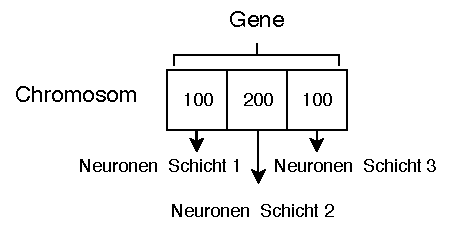
\includegraphics[scale=1.5]{img/gene_neuronen.pdf}
  \caption{Beispielhafte Zeichnung des Chromosom eines Individuums in welchem die Neuronen als Gene realisiert wurden}
  \label{fig:gene_neuronen}
\end{figure}

\subsection{Auswertung}
Alle Ergebnisse werden automatisch mit den dazugehörigen Konfigurationen und Berechnungen in einer Json-Datei abgespeichert. Aus dieser Json-Datei wird dann automatisch eine Zusammenfassung aller Ergebnisse erstellt und anschließend in einer Excel Datei abgespeichert. Des Weiteren werden Dichte Diagramme aus den Json-Dateien zu den einzelnen Hyperparametern automatisch erstellt und gespeichert. In diesen werden die Dichteverteilungen der einzelnen Hyperparameter in Bezug auf die Fitness dargestellt. Somit können die Hyperparameter intuitiv ausgewählt werden. Der Ablauf der Auswertung ist schematisch in Abbildung \ref{fig:implementierung_auswertung} abgebildet. 

\begin{figure}[H]
  \centering  
  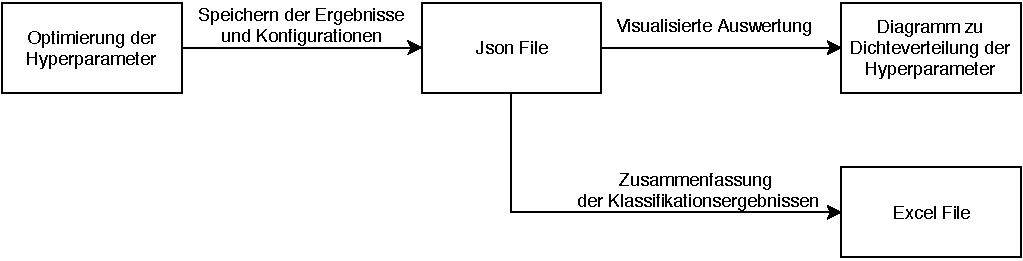
\includegraphics[scale=0.9]{img/Auswertung.pdf}
  \caption{Datenstruktur der Auswertung}
  \label{fig:implementierung_auswertung}
\end{figure}


\section{Zusammenfassung}
In diesem Kapitel wurde auf die implementierten Optimierungsalgorithmen und künstlichen neuronalen Netzen eingegangen. Dazu wurde zuerst der Systemaufbau, Programmiersprache und alle dazu gehörigen Python-Pakete und ihre jeweilige Funktion erläutert. Nachfolgend wurde auf die Hardware, die zur Verfügung stand, eingegangen. Danach wurden die verwendeten Datensätze: Mnist Fashion, Mnist Digits und der Cifar10 Datensatz erklärt. Bei allen drei handelt es sich um Bilddatensätze, welche mit 28x28 Pixel und 32x32x3 Pixel, relativ kleine Bilddaten enthalten. Anschließend wird erläutert, welche 5 Schritte für den Genetischen Algorithmus implementiert wurden, sowie die Methoden, die zur Evaluierung des GA eingesetzt werden. Ebenso wird die implementierte Zufallssuche erläutert welche zum Vergleich des GA dient. Beide Algorithmen benutzen die gleichen Datensätze, als auch die gleichen künstlichen neuronalen Netze. Als KNNs werden ein Fully Conneted Netz mit zwei Variationen optimiert und ein Convolutional Neuronal Network verwendet. Zum Abspeichern der Netze werden Json und Excel Files benutzt. Aus diesen Files werden dann die Auswertungen bzw. das Dichte-Diagramm bestimmt.
\cleardoublepage

\chapter{Ergebnisse und Auswertung}
\section{Evaluation und Tests}
\subsection{Einleitung}

\subsection{Testszenarien}

\subsection{Evaluation}

\subsection{Ergebniss und Interpretation}

\subsection{Zusammenfassung}
\cleardoublepage

\chapter{Fazit und Ausblick}
\section{Fazit}
Mit Hinblick auf die zu Beginn der Arbeit definierten Ziele, kann ein abschließendes positives Fazit gezogen werden. Zur Umsetzung dieser Ziele wurde ein automatisierter Traininigs- und Auswerte- Prozess für künstliche neuronale Netze erstellt. Anschließend wurde ein Genetischer Algorithmus zur Optimierung von Hyperparametern künstlicher neuronaler Netze konzipiert. Dazu wurden Versuche durchgeführt, in welchen die Methoden des Genetischen Algorithmus verglichen wurden. Um diese Versuche durchzuführen, wurden alle State-of-the-Art Methoden implementiert. Die zielführendsten Methoden wurden anschließend in der Evaluierung verwendet. Des Weiteren wurde die Zufallssuche als Algorithmus zum Vergleichen der Ergebnisse ausgewählt und implementiert. Abschließend wurden diese beiden Algorithmen evaluiert. In den Ergebnissen zeigte der Genetische Algorithmus nicht die erhofften Verbesserungen in der Klassifikationsgenauigkeit gegenüber der Zufallssuche. Obwohl der Genetische Algorithmus wesentlich mehr Individuen findet die eine hohe Qualität aufweisen. Bei den Individuen des GA konnte sich jedoch kein Individuum deutlich von den anderen absetzen bzw. eine Verbesserung der Klassifikationsgenauigkeit erbringen. Dies liegt daran, dass kleine Veränderungen der Hyperparameter keine messbaren Unterschiede auf DIE Endergebnisse haben. Dennoch hat sich in der Evaluierung gezeigt, dass sich die Hyperparameter in einem bestimmten Intervall befinden müssen, sonst liefert das künstliche neuronale Netz keine brauchbaren Ergebnisse. Dieser bestimme Bereich kann über das Dichte-Diagramm des Genetischen Algorithmus sichtbar gemacht werden. Dieser Bereich ist für jedes Netz bzw. Modell-Architektur individuell und kann sogar von den Trainingsdaten abhängen. Der Genetische Algorithmus, ist in Bezug auf das Finden der besten Hyperparameter, vergleichbar mit der Zufallssuche. Zusätzlich hat der GA den Vorteil, dass er Zusatzinformationen besitzt. Somit kann er ein bestimmtes Intervall angeben, in welchem sich die Hyperparameter befinden müssen, um gute Ergebnisse zu erreichen. Zusammengefasst kann gesagt werden, dass bei einem kleinen Suchraum oder wenn nur wenig Rechenressourcen zur Verfügung stehen, eine Zufallssuche ausreichend ist. Doch wenn der Suchraum für die Hyperparameter groß ist oder ein leistungsstarker Rechner zur Verfügung steht, hat der Genetische Algorithmus durchaus seine Vorteile.


\section{Ausblick} \label{ausblick}
Die Optimierung von Hyperparametern mit Hilfe eines Genetischen Algorithmus hat nur bedingt Verbesserungen erbracht. Weswegen eine Optimierung der Hyperparameter mit Hilfe eines anderen Optimierungsalgorithmus denkbar wäre. Hierfür ist eine Optimierung mit dem Bayesian Optimierer oder dem HyperOPt (Distributed Asynchronous Hyper-parameter Optimization) denkbar. 

Neben der Optimierung von Hyperparametern könnte in einer weiteren Arbeit auf die Optimierung der Modell-Architektur eingegangen werden. Zu diesem Thema wurden in dieser Arbeit bereits erste Versuche durchgeführt. Die Ergebnisse des Versuches \ref{versuch_modell} zeigten bei der Optimierung eine Tendenz zu größeren Modell-Architekturen. Um dieser Tendenz entgegenzuwirken müsste eine geeignete Fitnessfunktion entwickelt werden. Hierfür könnte beispielsweise die Gesamtanzahl an Parametern als negativer Faktor mit einbezogen werden. Generell ist ein Finden spezieller Netze über das Erstellen einer speziellen Fitnessfunktion möglich. Eine spezielle Fintessfunktion ist nicht nur für die trainierbaren Parameter denkbar. Sie könnte auch zur Findung von Netzen mit hoher Interferenz genutzt werden. 

Zudem könnten noch andere Parameter als Gene umgesetzt werden. In dieser Arbeit ging es nur um die gängigen Hyperparameter \ref{sec:Grundlagen_Hyperparamete}. Diese Hyperparameter haben aber nur einen geringen Einfluss auf das Klassifizierungsergebnis. Es wäre durchaus denkbar eine Optimierung mit anderen oder mehreren Parametern durchzuführen. Somit kann der Genetische Algortihmus seine Vorteile im großen Suchraum ausspielen.

\cleardoublepage

%Literaturverzeichnis
\bibliographystyle{alpha}
\bibliography{Literatur}


\chapter{Anhang}
\section{Dichte-Diagramme zu den durchgeführten Optimierungen mit dem gesamten Datensatz}

\subsection{50 Iterationen des Genetischen Algorithmus des kleinen Fully-Connected Netzes}
\begin{figure}[H]
  \centering  
  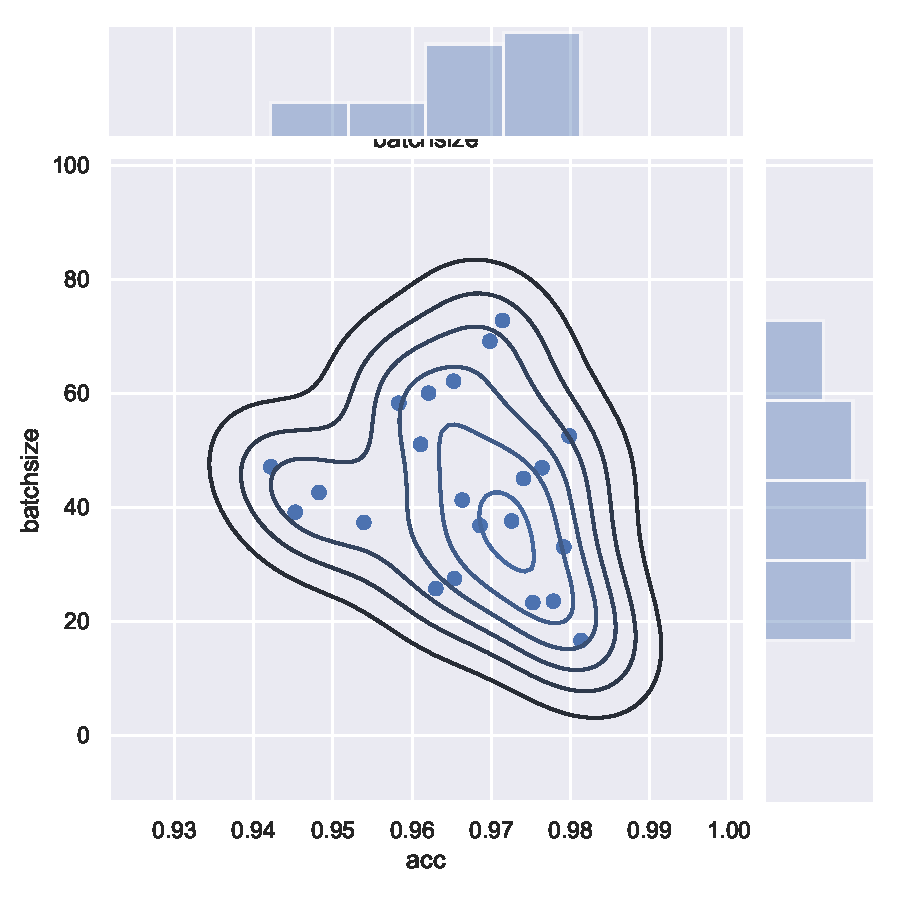
\includegraphics[scale=0.5]{anhang/GA_50_mnist_digits_False_small_jointplot_batchsize.pdf}
  \caption{Dichte-Diagramm der Batchsize in Verbindung mit der Klassifizierungsgenauigkeit(acc)}
  
\end{figure}

\begin{figure}[H]
  \centering  
  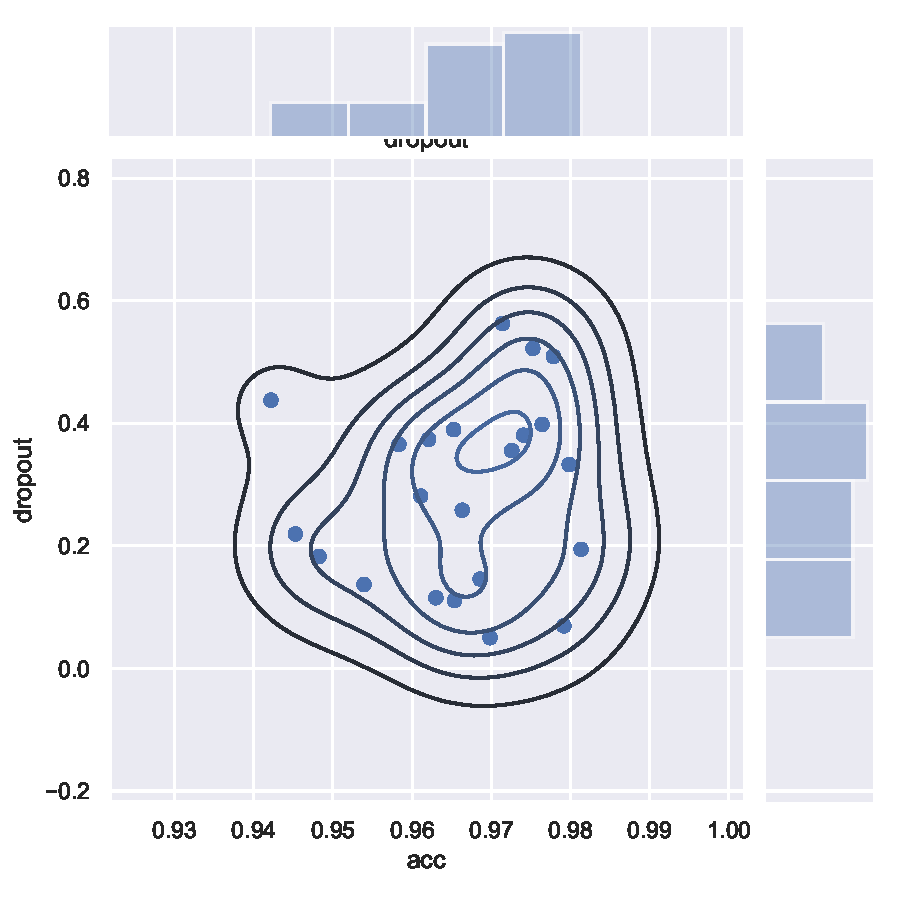
\includegraphics[scale=0.5]{anhang/GA_50_mnist_digits_False_small_jointplot_dropout.pdf}
  \caption{Dichte-Diagramm des Dropouts in Verbindung mit der Klassifizierungsgenauigkeit(acc)}
  
\end{figure}

\begin{figure}[H]
  \centering  
  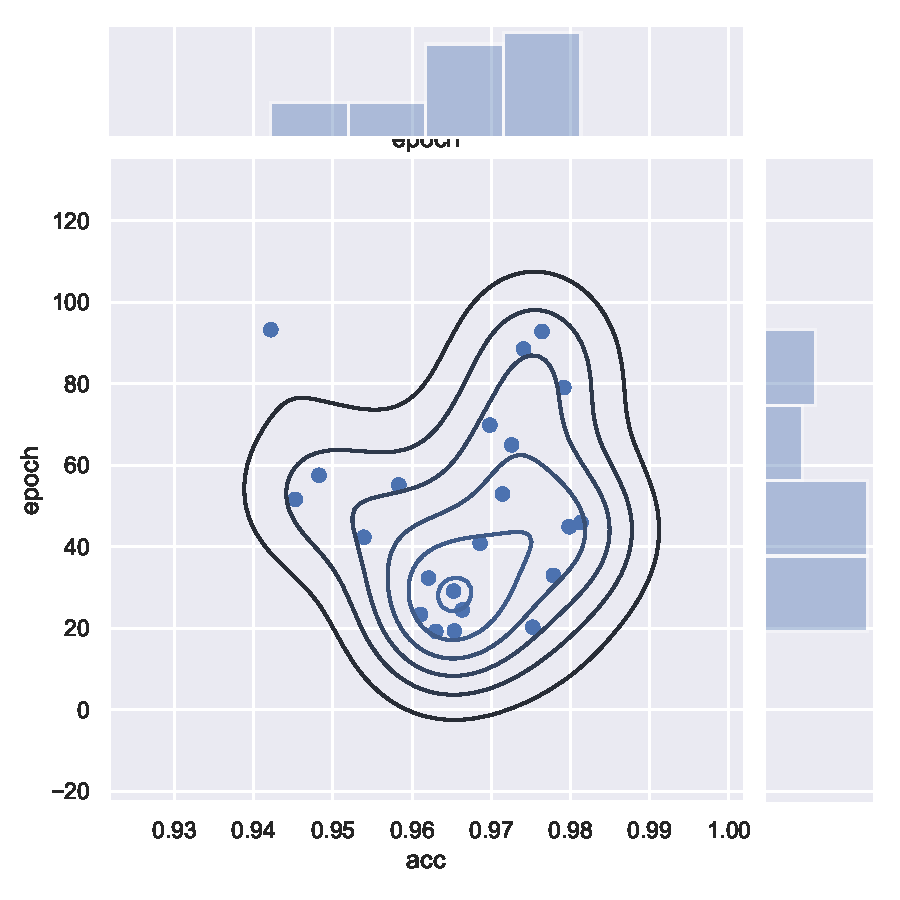
\includegraphics[scale=0.5]{anhang/GA_50_mnist_digits_False_small_jointplot_epoch.pdf}
  \caption{Dichte-Diagramm der Epochenanzahl in Verbindung mit der Klassifizierungsgenauigkeit(acc)}
  
\end{figure}

\begin{figure}[H]
  \centering  
  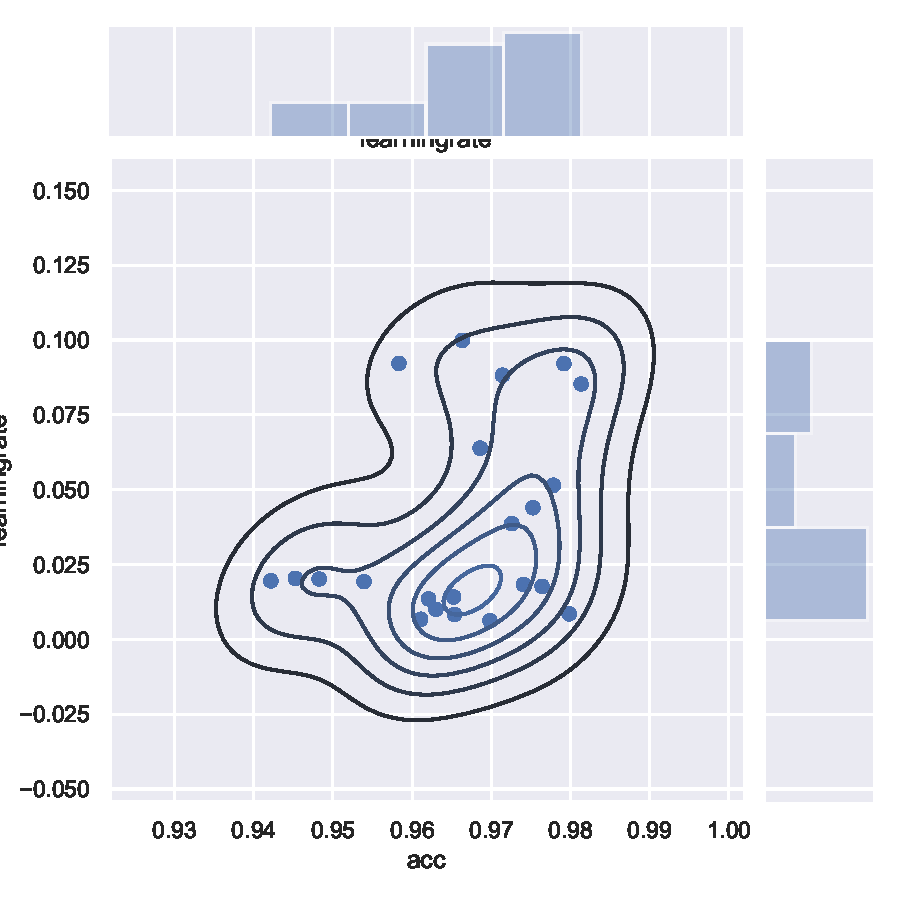
\includegraphics[scale=0.5]{anhang/GA_50_mnist_digits_False_small_jointplot_learningrate.pdf}
  \caption{Dichte-Diagramm der Lernrate in Verbindung mit der Klassifizierungsgenauigkeit(acc)}
  
\end{figure}

\begin{figure}[H]
  \centering  
  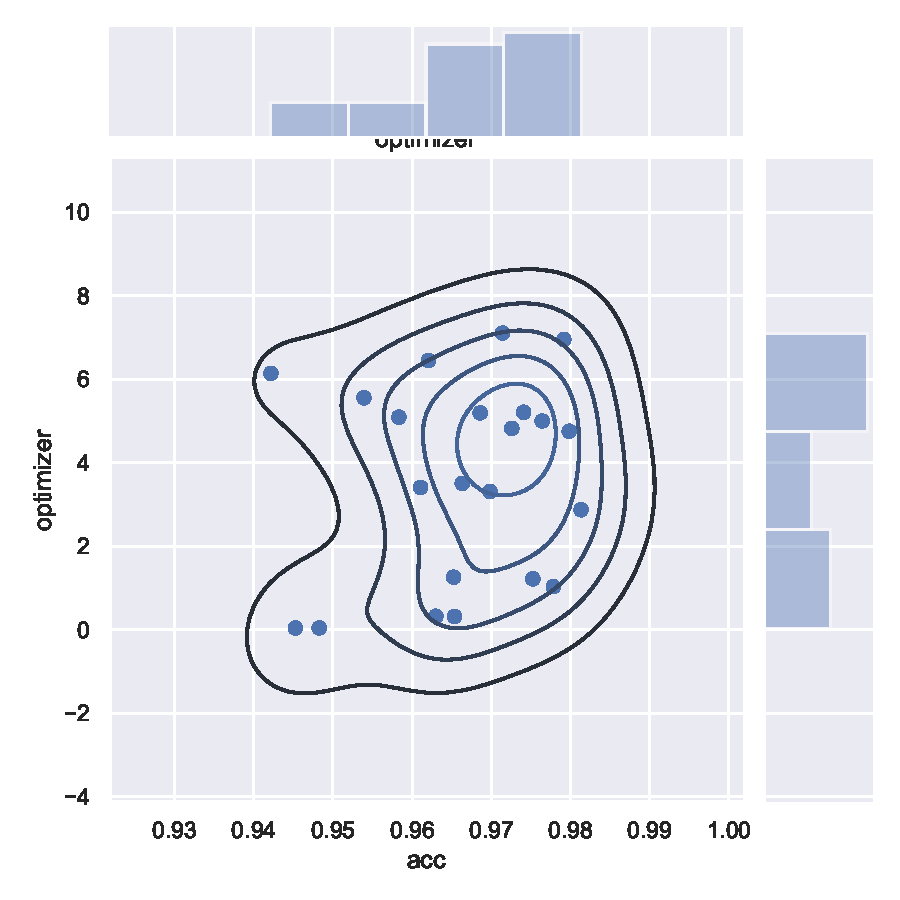
\includegraphics[scale=0.5]{anhang/GA_50_mnist_digits_False_small_jointplot_optimizer.pdf}
  \caption{Dichte-Diagramm des Optimierers in Verbindung mit der Klassifizierungsgenauigkeit(acc)}
  
\end{figure}

\subsection{50 Iterationen des Genetischen Algorithmus des großen Fully-Connected Netzes}
\begin{figure}[H]
  \centering  
  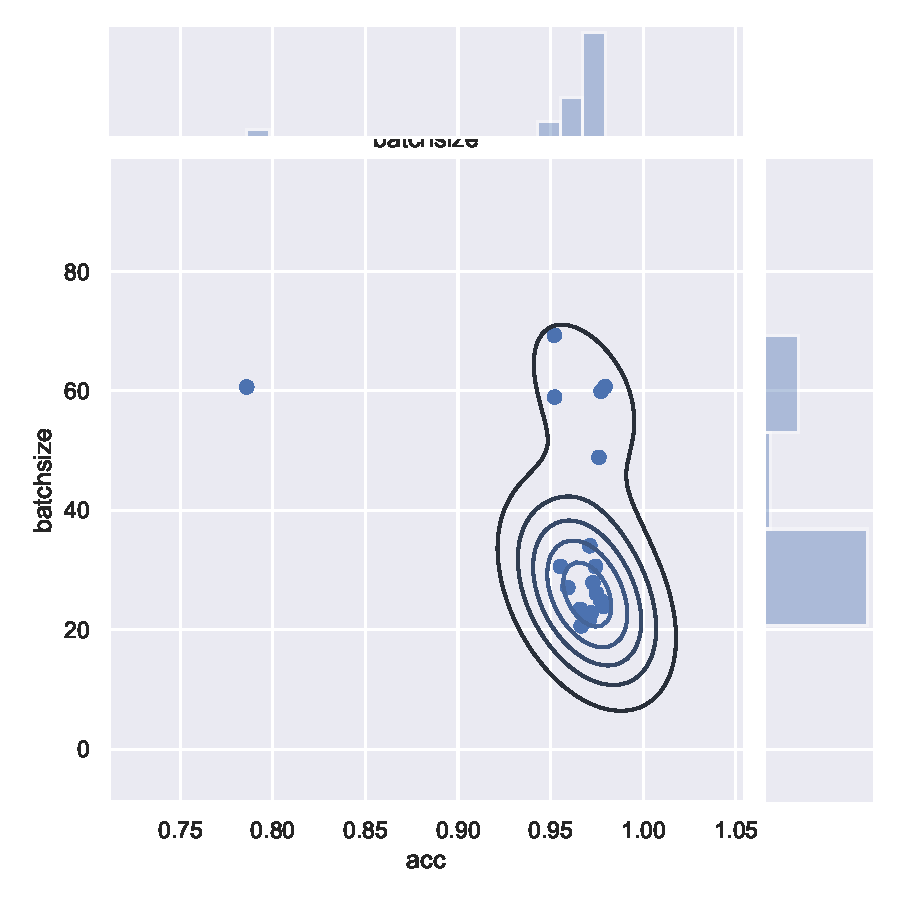
\includegraphics[scale=0.5]{anhang/GA_50_mnist_digits_False_big_jointplot_batchsize.pdf}
  \caption{Dichte-Diagramm der Batchsize in Verbindung mit der Klassifizierungsgenauigkeit(acc)}
  
\end{figure}

\begin{figure}[H]
  \centering  
  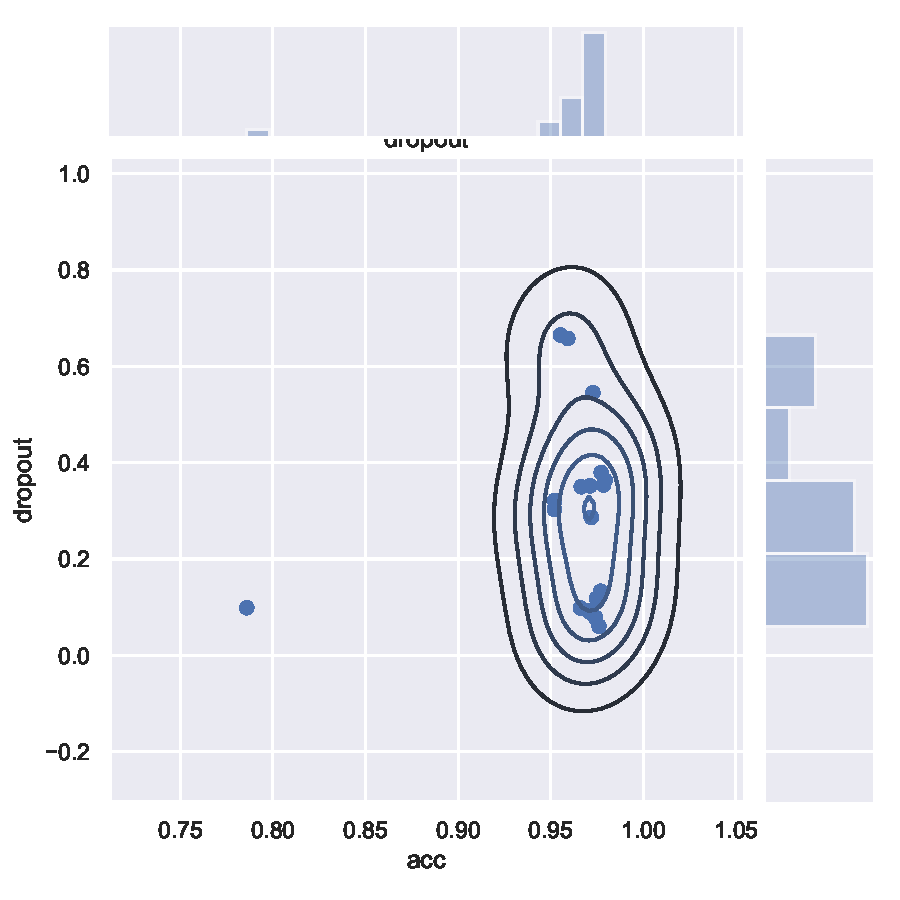
\includegraphics[scale=0.5]{anhang/GA_50_mnist_digits_False_big_jointplot_dropout.pdf}
  \caption{Dichte-Diagramm des Dropouts in Verbindung mit der Klassifizierungsgenauigkeit(acc)}
  
\end{figure}

\begin{figure}[H]
  \centering  
  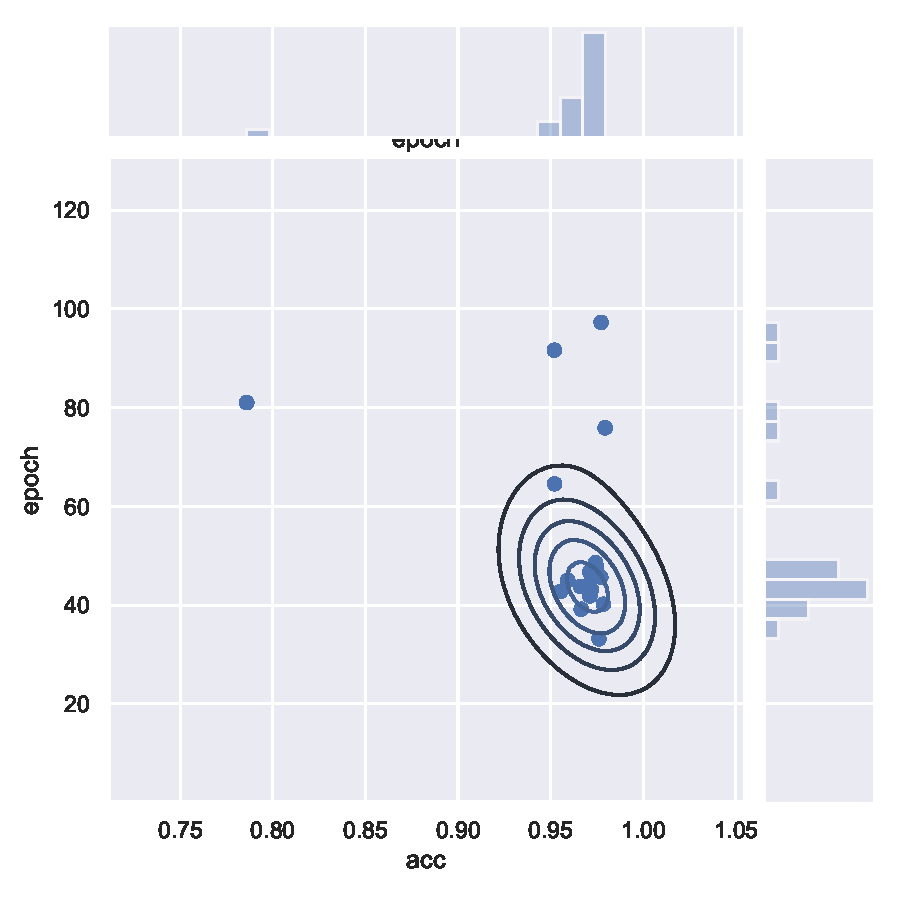
\includegraphics[scale=0.5]{anhang/GA_50_mnist_digits_False_big_jointplot_epoch.pdf}
  \caption{Dichte-Diagramm der Epochenanzahl in Verbindung mit der Klassifizierungsgenauigkeit(acc)}
  
\end{figure}

\begin{figure}[H]
  \centering  
  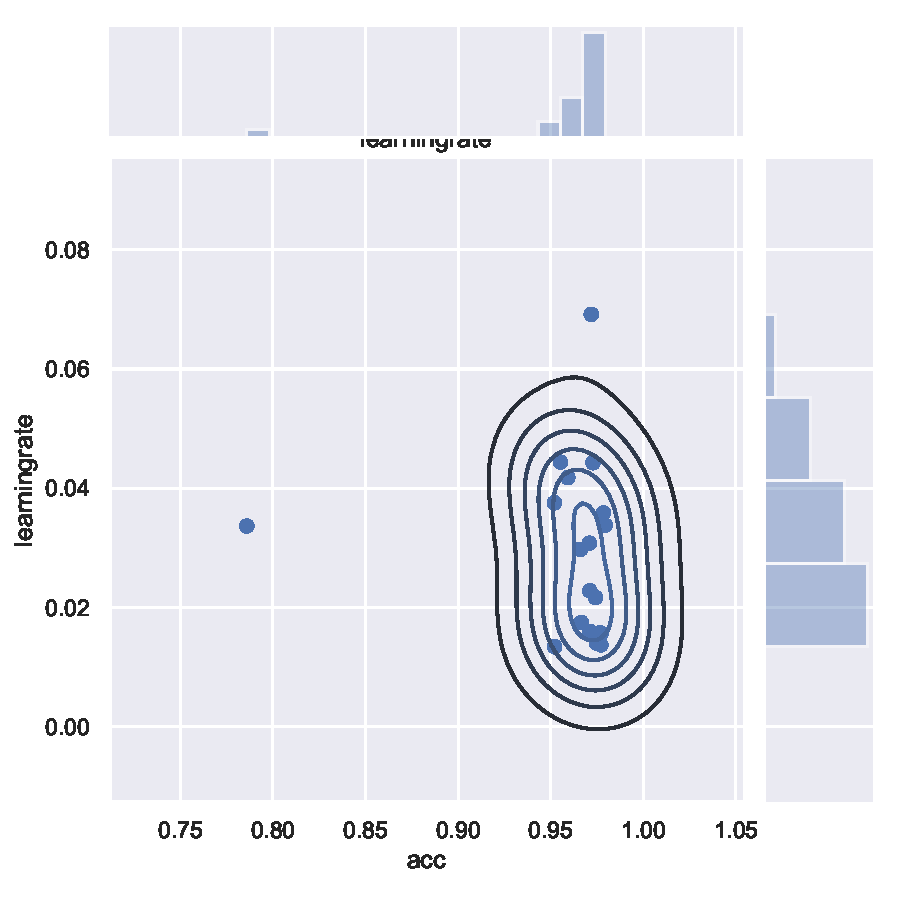
\includegraphics[scale=0.5]{anhang/GA_50_mnist_digits_False_big_jointplot_learningrate.pdf}
  \caption{Dichte-Diagramm der Lernrate in Verbindung mit der Klassifizierungsgenauigkeit(acc)}
  
\end{figure}

\begin{figure}[H]
  \centering  
  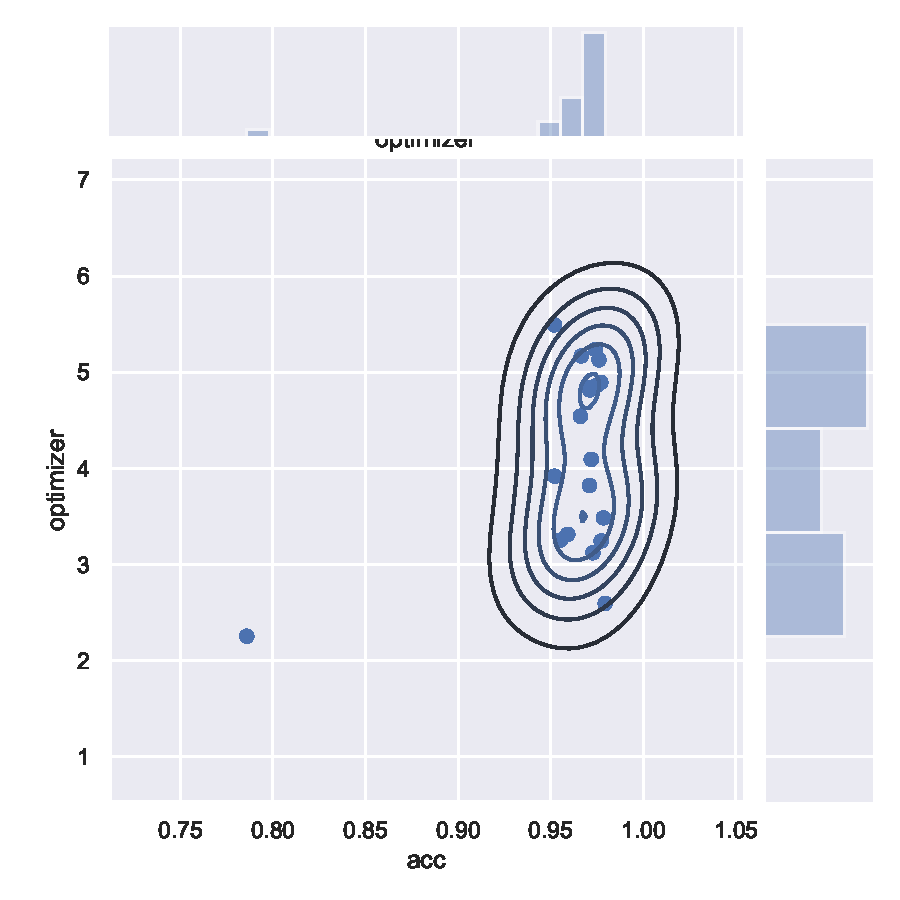
\includegraphics[scale=0.5]{anhang/GA_50_mnist_digits_False_big_jointplot_optimizer.pdf}
  \caption{Dichte-Diagramm des Optimierers in Verbindung mit der Klassifizierungsgenauigkeit(acc)}
  
\end{figure}


\subsection{250 Iterationen des Genetischen Algorithmus des kleinen Fully-Connected Netzes}
\begin{figure}[H]
  \centering  
  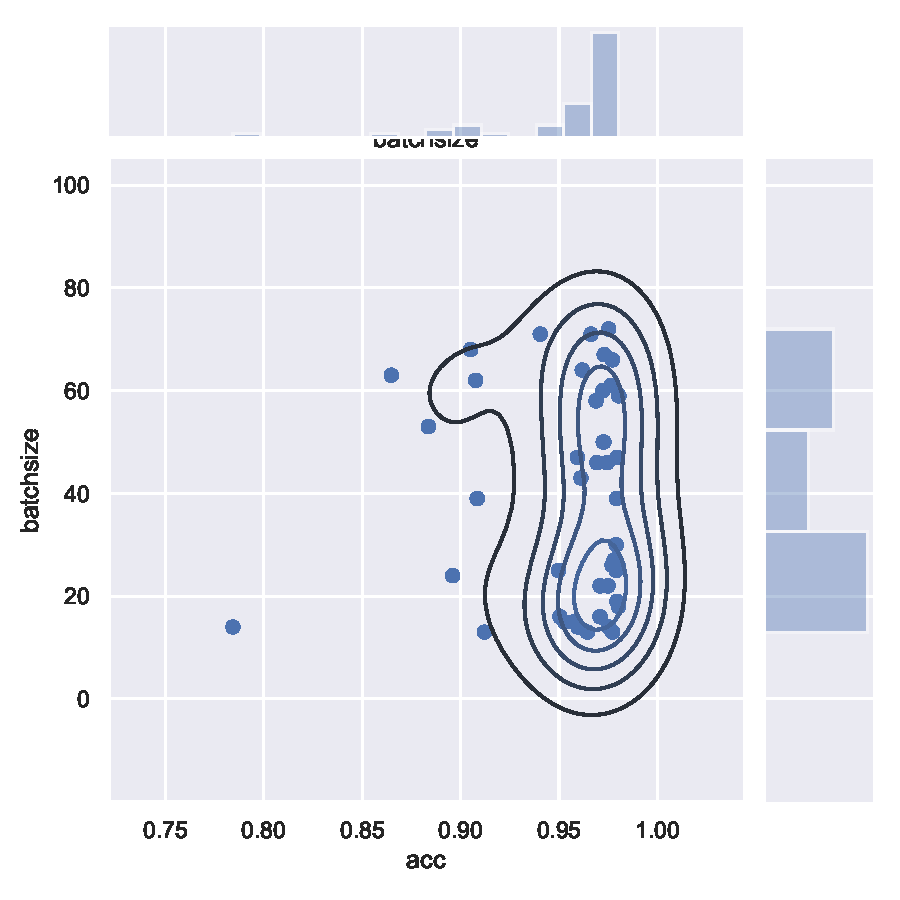
\includegraphics[scale=0.5]{anhang/GA_250_mnist_digits_False_small_jointplot_batchsize.pdf}
  \caption{Dichte-Diagramm der Batchsize in Verbindung mit der Klassifizierungsgenauigkeit(acc)}
  
\end{figure}

\begin{figure}[H]
  \centering  
  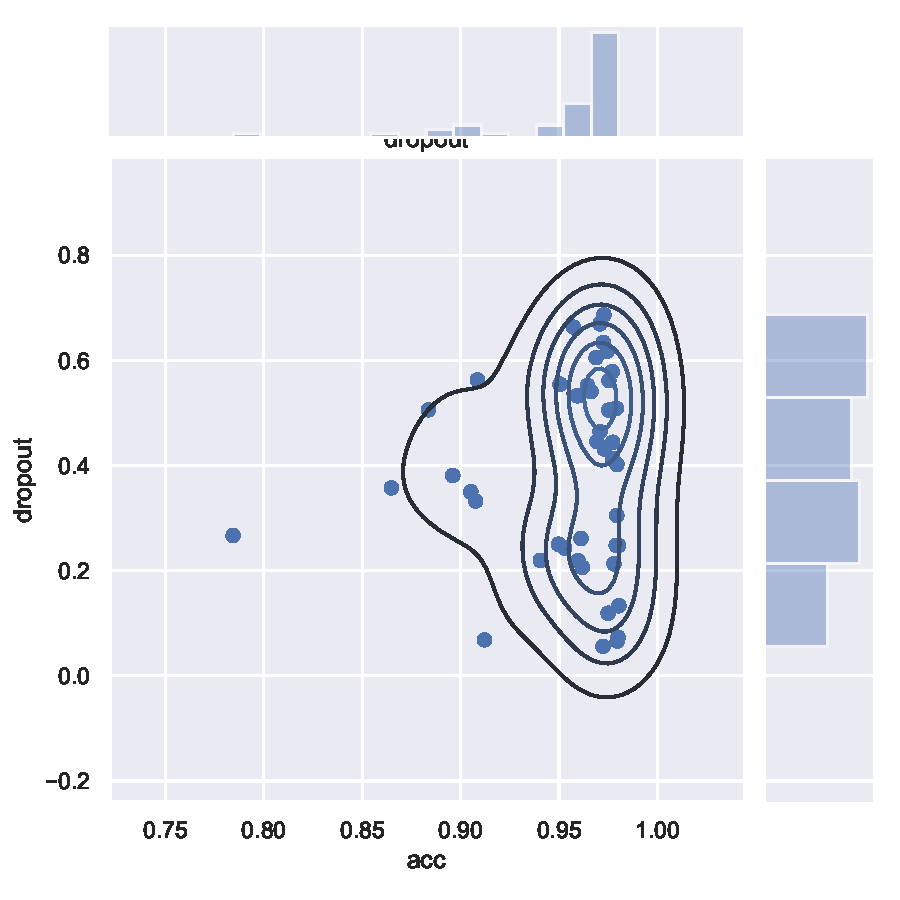
\includegraphics[scale=0.5]{anhang/GA_250_mnist_digits_False_small_jointplot_dropout.pdf}
  \caption{Dichte-Diagramm des Dropouts in Verbindung mit der Klassifizierungsgenauigkeit(acc)}
  
\end{figure}

\begin{figure}[H]
  \centering  
  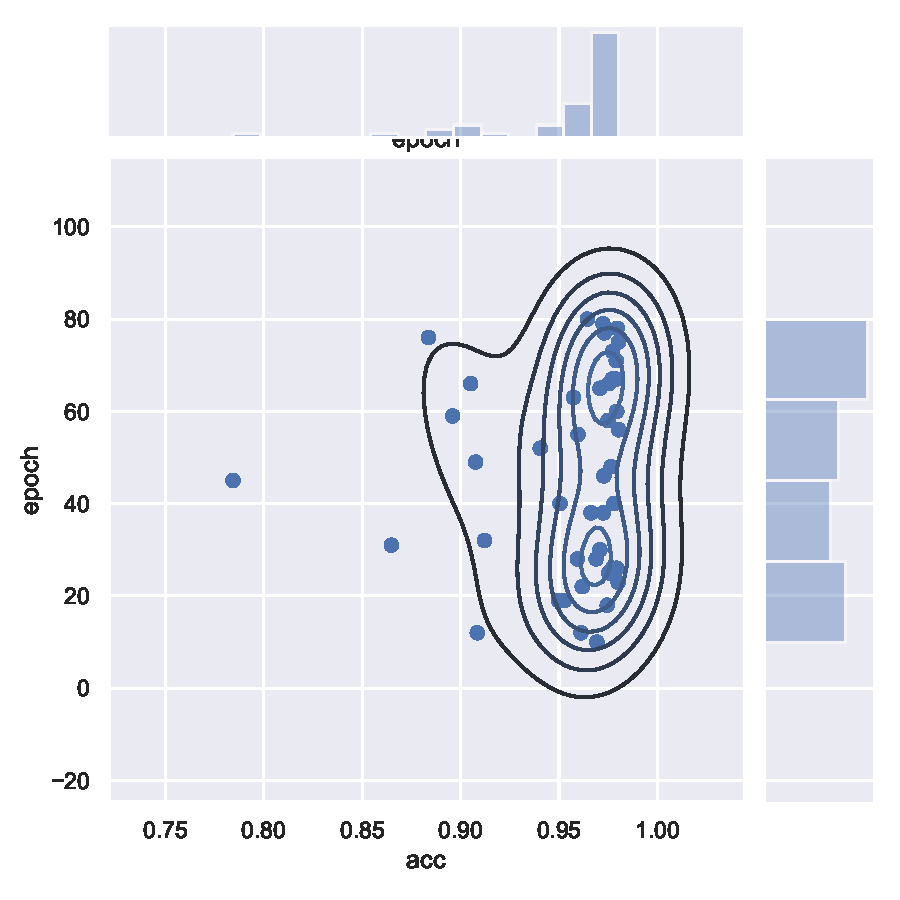
\includegraphics[scale=0.5]{anhang/GA_250_mnist_digits_False_small_jointplot_epoch.pdf}
  \caption{Dichte-Diagramm der Epochenanzahl in Verbindung mit der Klassifizierungsgenauigkeit(acc)}
  
\end{figure}

\begin{figure}[H]
  \centering  
  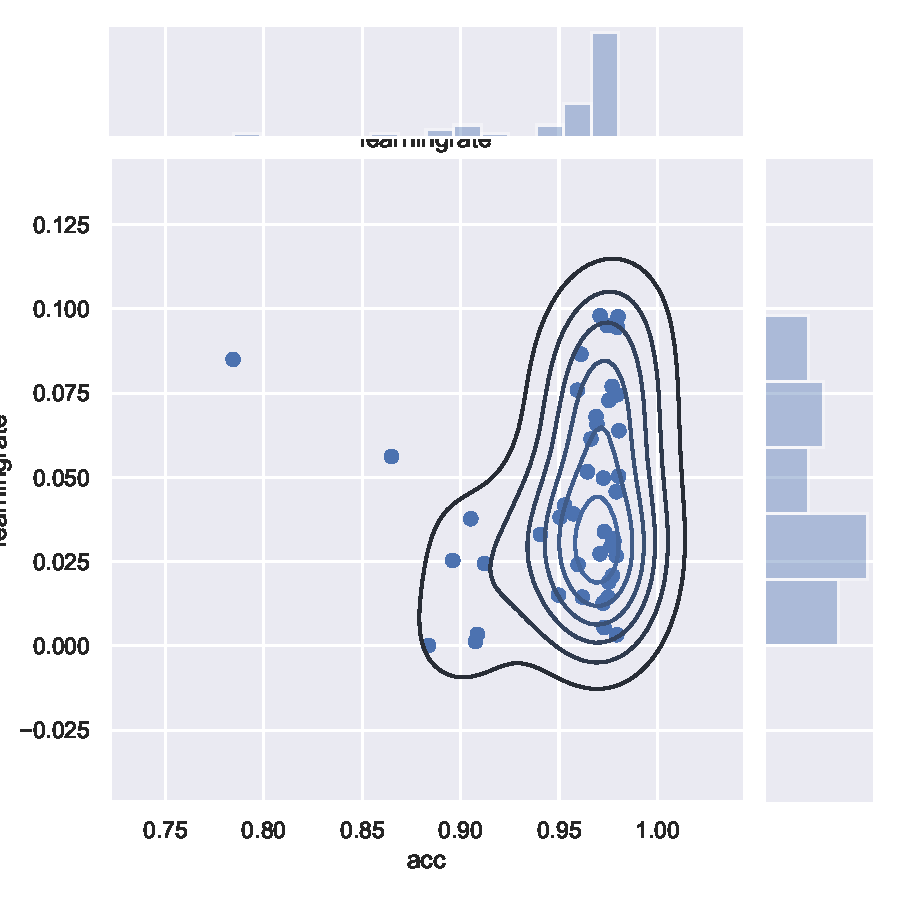
\includegraphics[scale=0.5]{anhang/GA_250_mnist_digits_False_small_jointplot_learningrate.pdf}
  \caption{Dichte-Diagramm der Lernrate in Verbindung mit der Klassifizierungsgenauigkeit(acc)}
  
\end{figure}

\begin{figure}[H]
  \centering  
  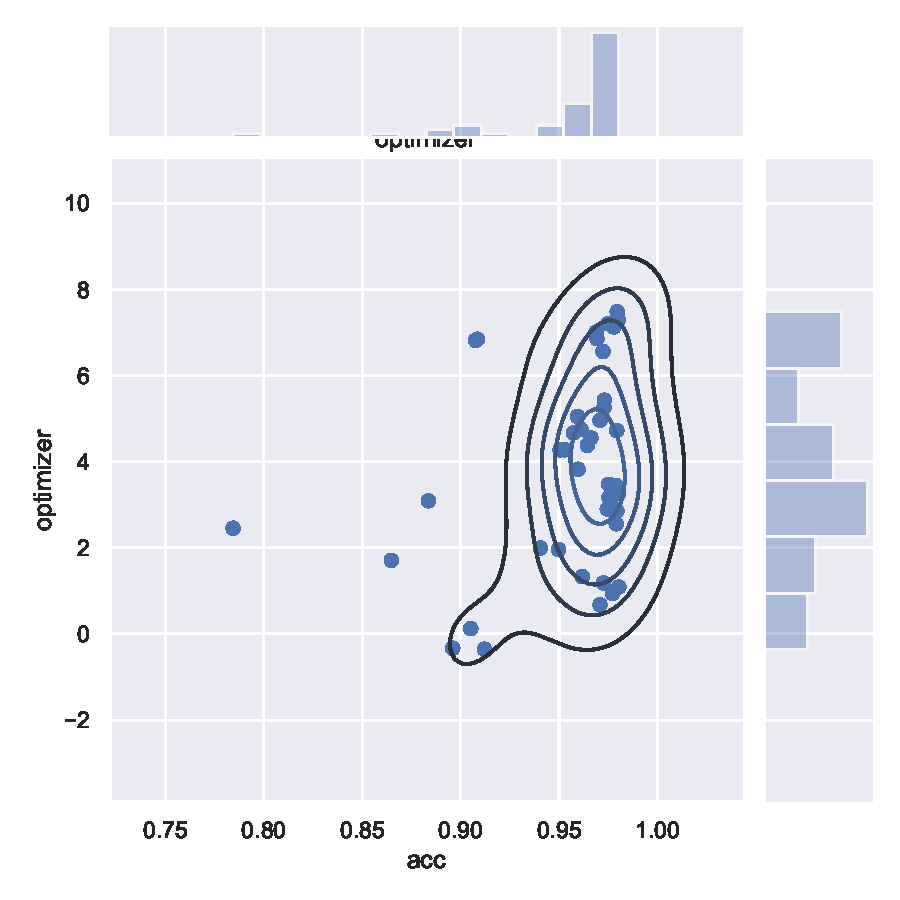
\includegraphics[scale=0.5]{anhang/GA_250_mnist_digits_False_small_jointplot_optimizer.pdf}
  \caption{Dichte-Diagramm des Optimierers in Verbindung mit der Klassifizierungsgenauigkeit(acc)}
  
\end{figure}

\subsection{250 Iterationen des Genetischen Algorithmus des großen Fully-Connected Netzes}
\begin{figure}[H]
  \centering  
  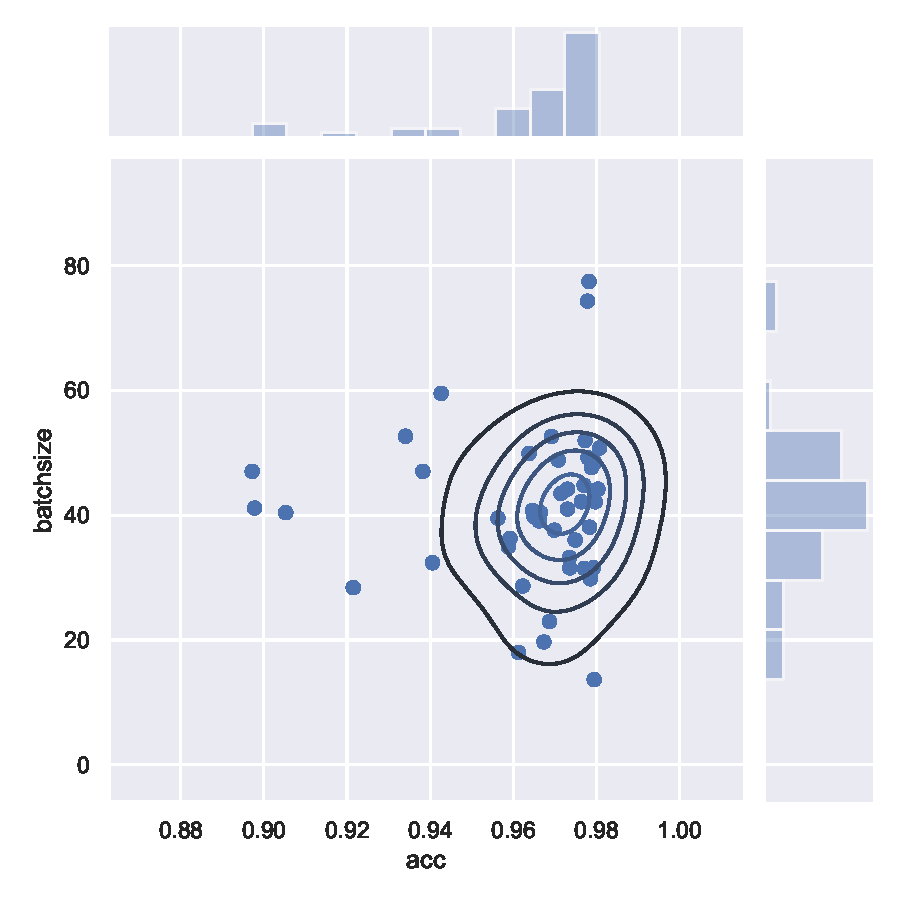
\includegraphics[scale=0.5]{anhang/GA_250_mnist_digits_False_big_jointplot_batchsize.pdf}
  \caption{Dichte-Diagramm der Batchsize in Verbindung mit der Klassifizierungsgenauigkeit(acc)}
  
\end{figure}

\begin{figure}[H]
  \centering  
  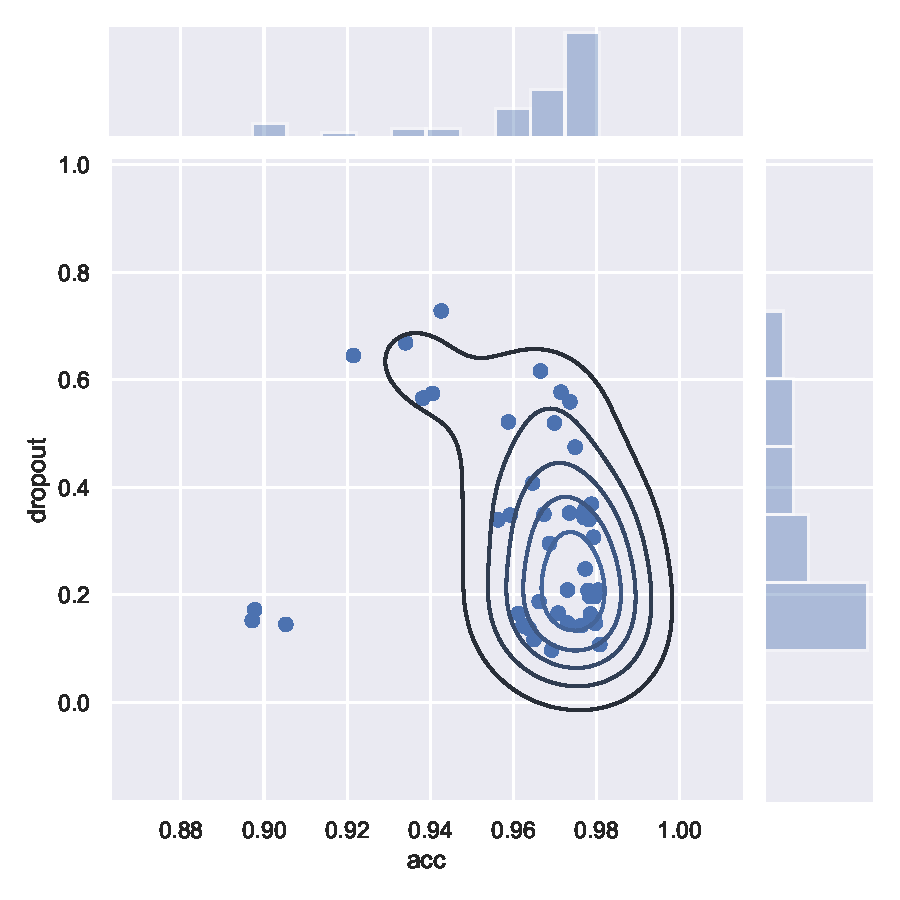
\includegraphics[scale=0.5]{anhang/GA_250_mnist_digits_False_big_jointplot_dropout.pdf}
  \caption{Dichte-Diagramm des Dropouts in Verbindung mit der Klassifizierungsgenauigkeit(acc)}
  
\end{figure}

\begin{figure}[H]
  \centering  
  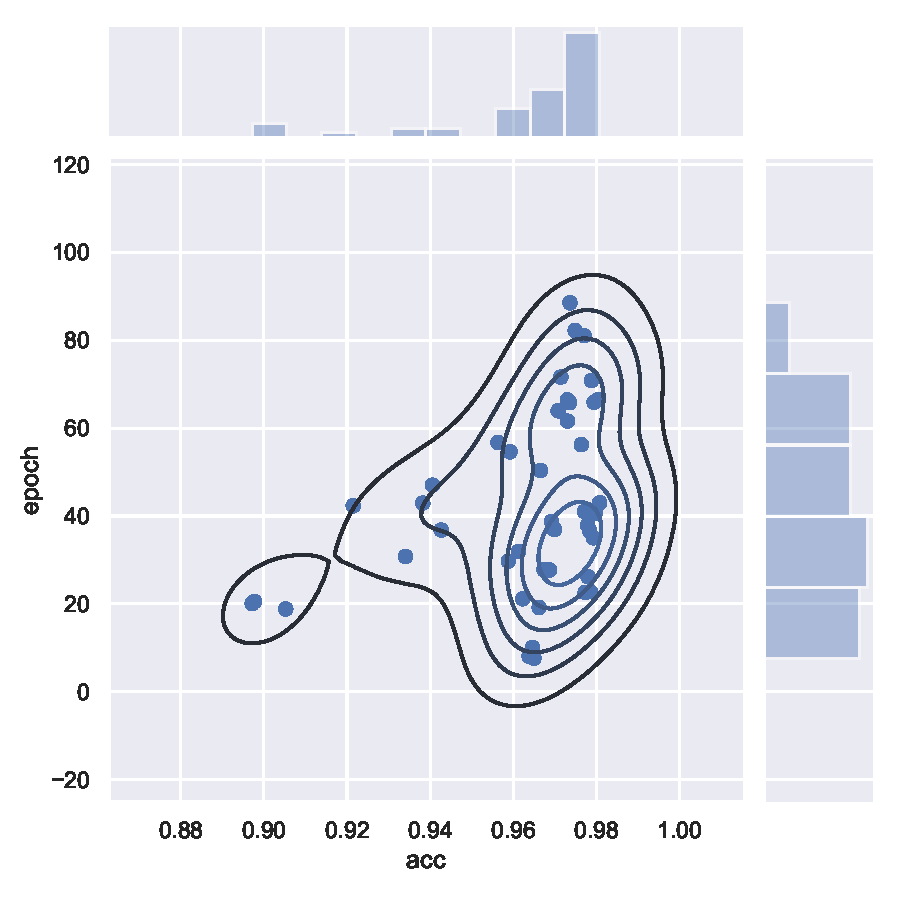
\includegraphics[scale=0.5]{anhang/GA_250_mnist_digits_False_big_jointplot_epoch.pdf}
  \caption{Dichte-Diagramm der Epochenanzahl in Verbindung mit der Klassifizierungsgenauigkeit(acc)}
  
\end{figure}

\begin{figure}[H]
  \centering  
  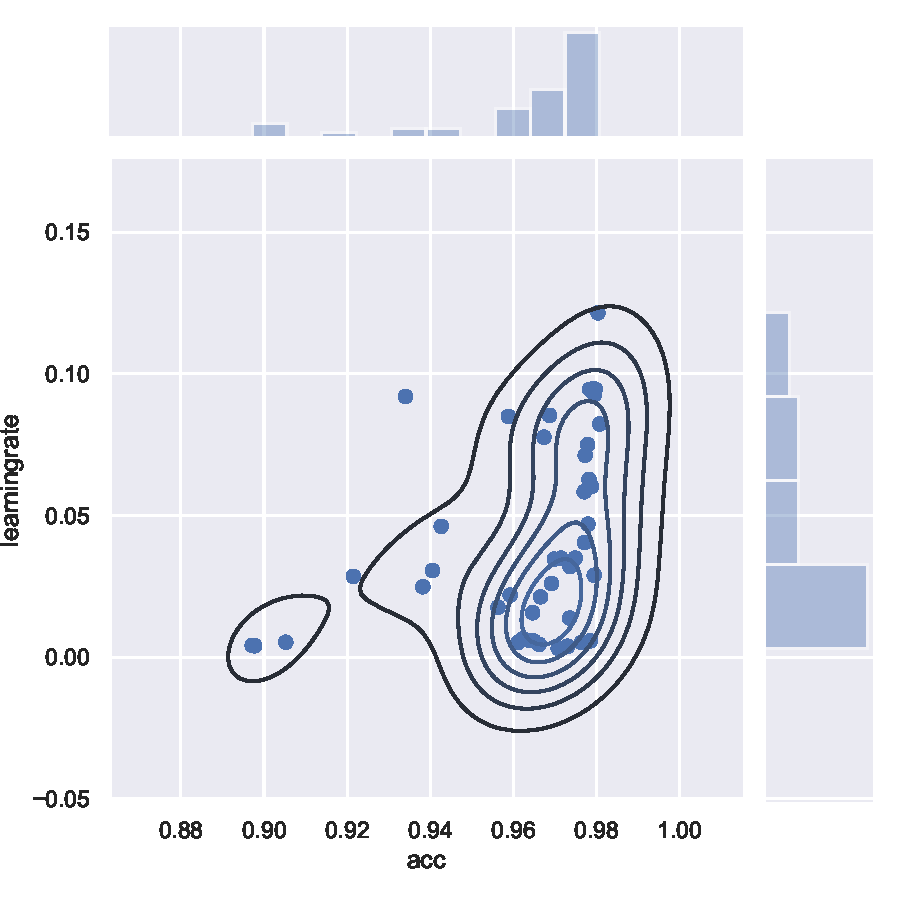
\includegraphics[scale=0.5]{anhang/GA_250_mnist_digits_False_big_jointplot_learningrate.pdf}
  \caption{Dichte-Diagramm der Lernrate in Verbindung mit der Klassifizierungsgenauigkeit(acc)}
  
\end{figure}

\begin{figure}[H]
  \centering  
  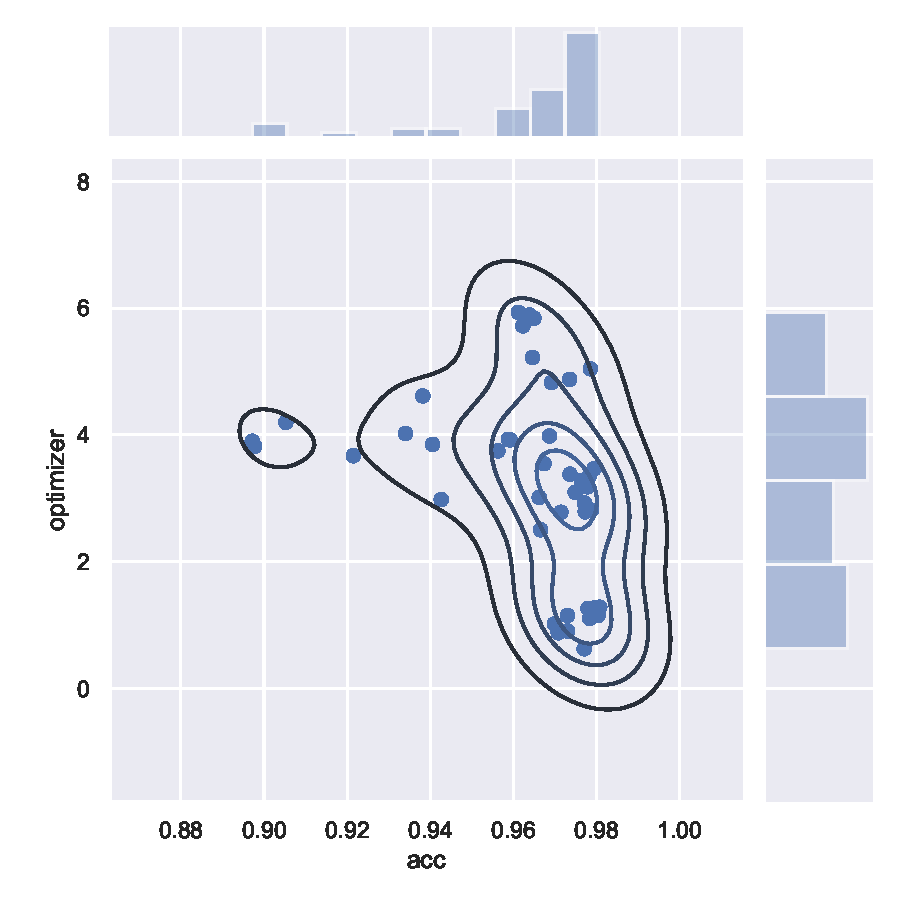
\includegraphics[scale=0.5]{anhang/GA_250_mnist_digits_False_big_jointplot_optimizer.pdf}
  \caption{Dichte-Diagramm des Optimierers in Verbindung mit der Klassifizierungsgenauigkeit(acc)}
  
\end{figure}

\subsection{50 Iterationen des Genetischen Algorithmus des Convolutional Neural Network}
\begin{figure}[H]
  \centering  
  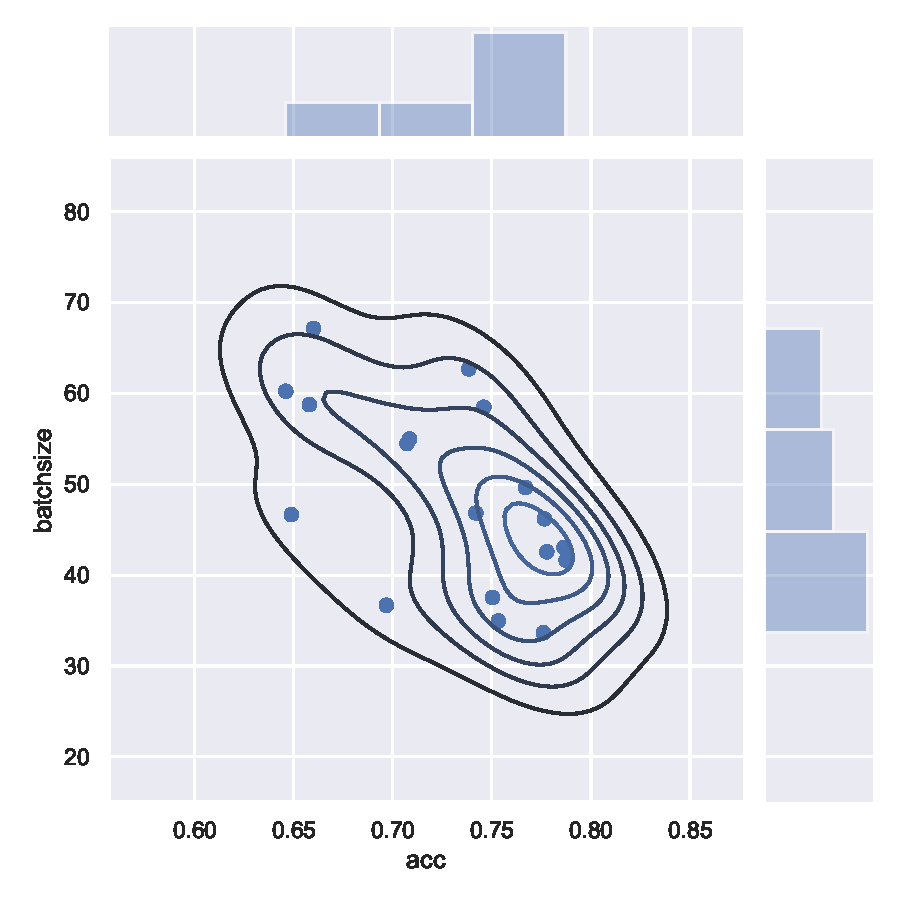
\includegraphics[scale=0.5]{anhang/GA_50_cifar10_False_big_jointplot_batchsize.pdf}
  \caption{Dichte-Diagramm der Batchsize in Verbindung mit der Klassifizierungsgenauigkeit(acc)}
  
\end{figure}

\begin{figure}[H]
  \centering  
  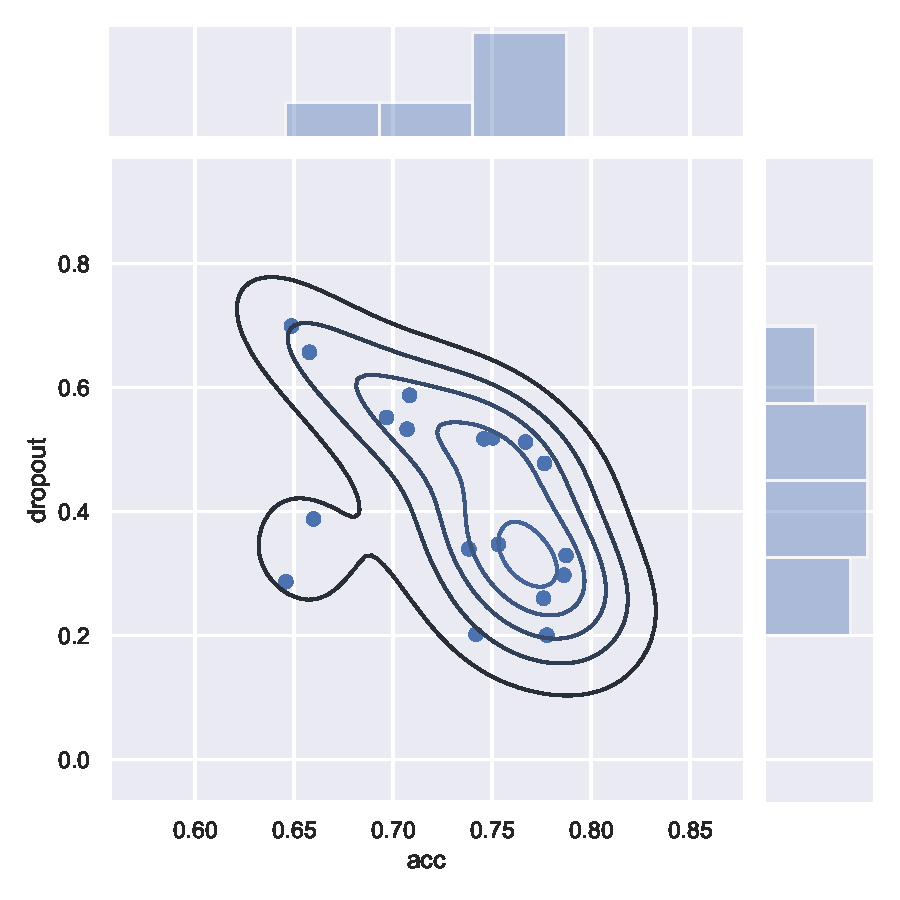
\includegraphics[scale=0.5]{anhang/GA_50_cifar10_False_big_jointplot_dropout.pdf}
  \caption{Dichte-Diagramm des Dropouts in Verbindung mit der Klassifizierungsgenauigkeit(acc)}
  
\end{figure}

\begin{figure}[H]
  \centering  
  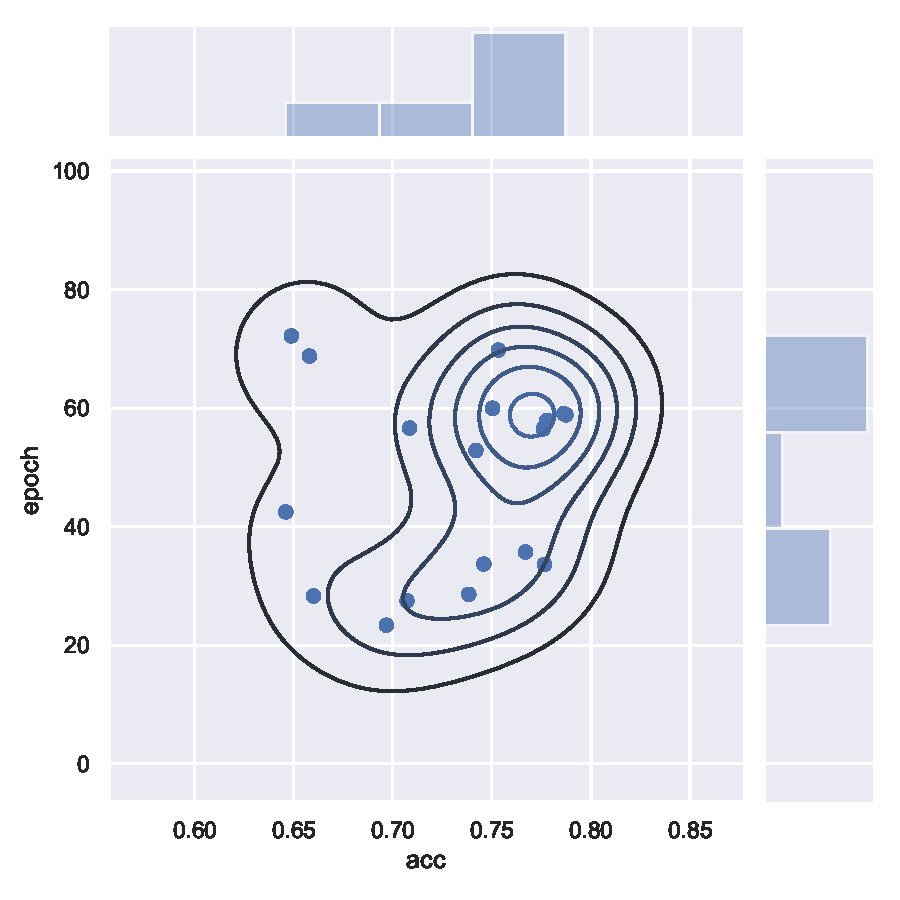
\includegraphics[scale=0.5]{anhang/GA_50_cifar10_False_big_jointplot_epoch.pdf}
  \caption{Dichte-Diagramm der Epochenanzahl in Verbindung mit der Klassifizierungsgenauigkeit(acc)}
  
\end{figure}

\begin{figure}[H]
  \centering  
  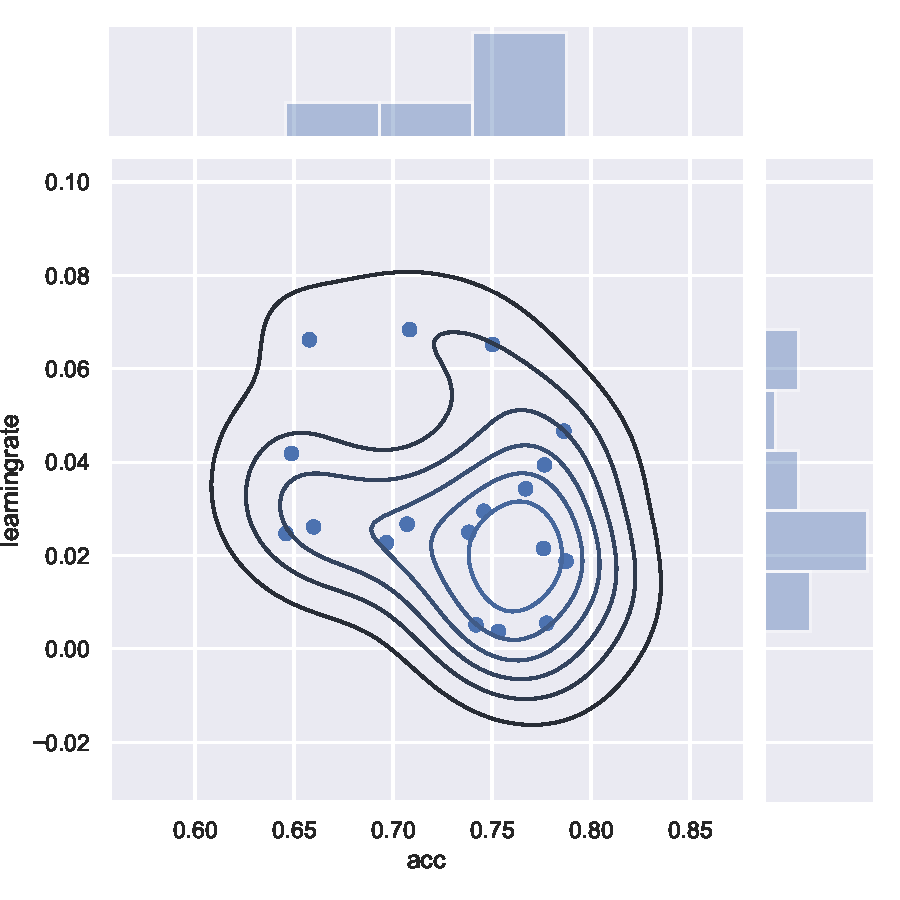
\includegraphics[scale=0.5]{anhang/GA_50_cifar10_False_big_jointplot_learningrate.pdf}
  \caption{Dichte-Diagramm der Lernrate in Verbindung mit der Klassifizierungsgenauigkeit(acc)}
  
\end{figure}

\begin{figure}[H]
  \centering  
  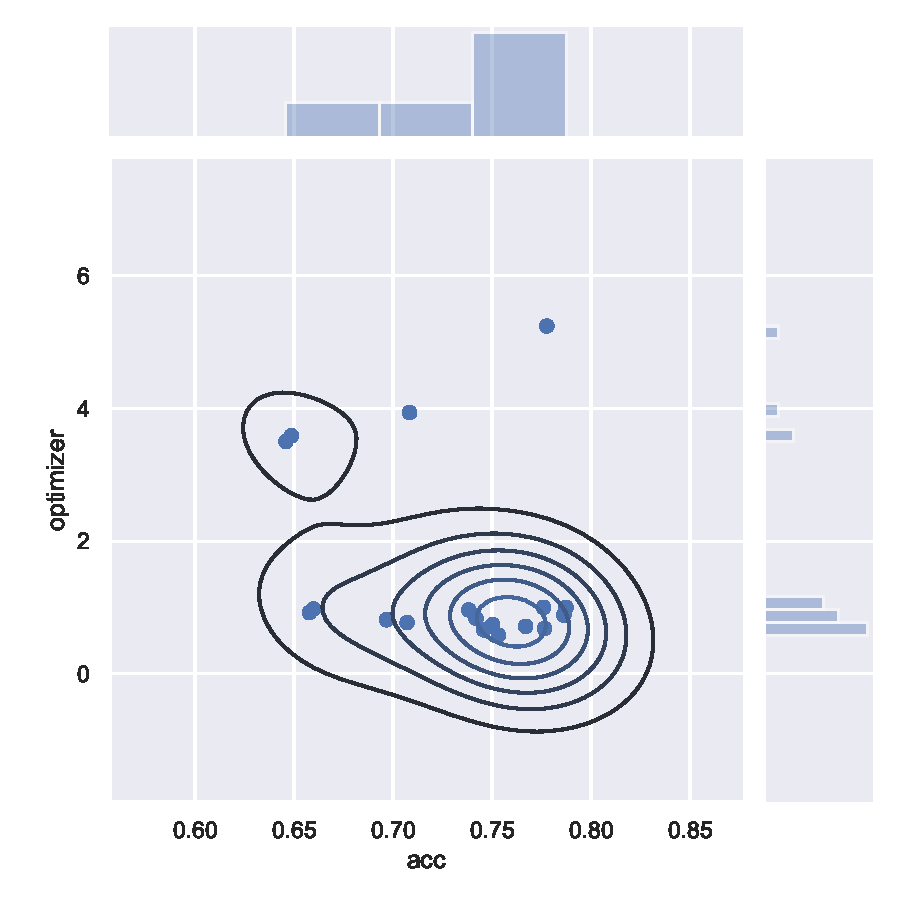
\includegraphics[scale=0.5]{anhang/GA_50_cifar10_False_big_jointplot_optimizer.pdf}
  \caption{Dichte-Diagramm des Optimierers in Verbindung mit der Klassifizierungsgenauigkeit(acc)}
\end{figure}

\subsection{250 Iterationen des Genetischen Algorithmus des Convolutional Neural Network}
\begin{figure}[H]
  \centering  
  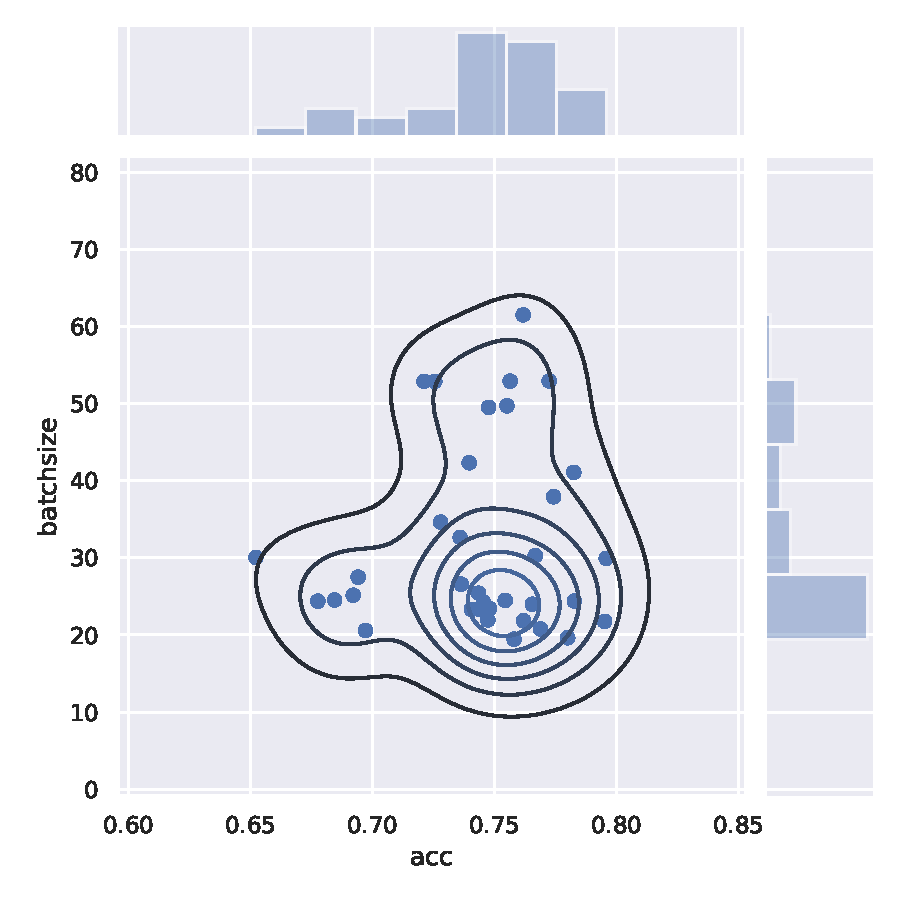
\includegraphics[scale=0.5]{anhang/GA_250_cifar10_False_big_jointplot_batchsize.pdf}
  \caption{Dichte-Diagramm der Batchsize in Verbindung mit der Klassifizierungsgenauigkeit(acc)}
\end{figure}

\begin{figure}[H]
  \centering  
  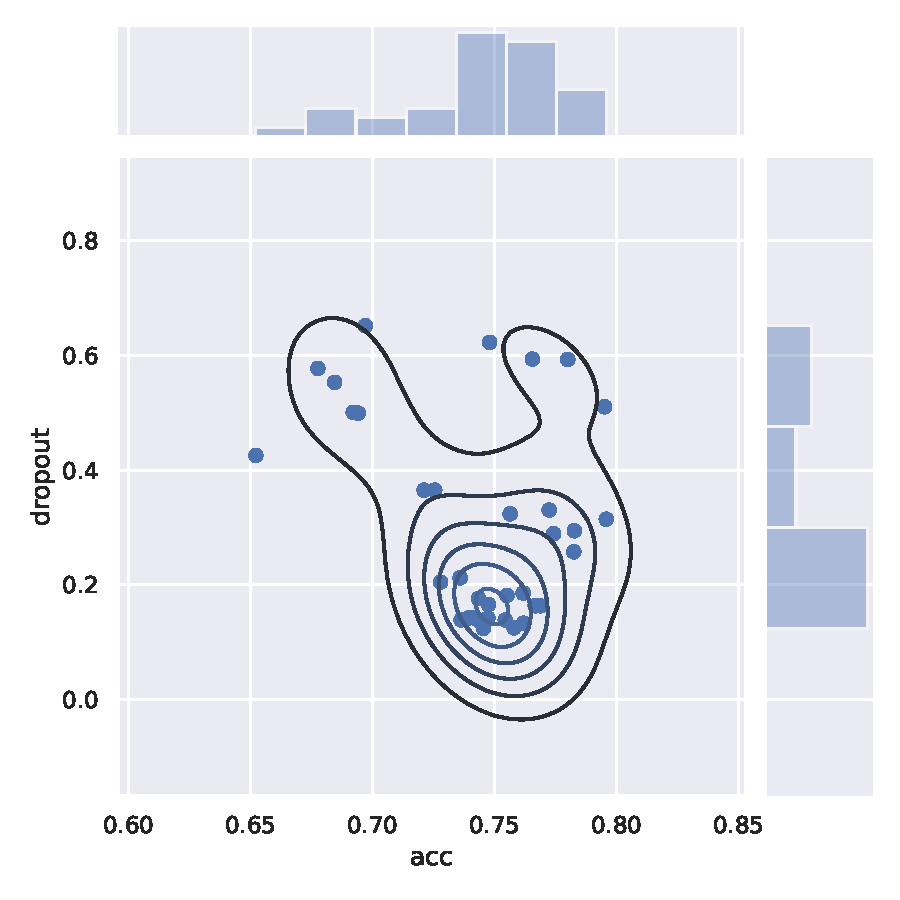
\includegraphics[scale=0.5]{anhang/GA_250_cifar10_False_big_jointplot_dropout.pdf}
  \caption{Dichte-Diagramm des Dropouts in Verbindung mit der Klassifizierungsgenauigkeit(acc)}
\end{figure}

\begin{figure}[H]
  \centering  
  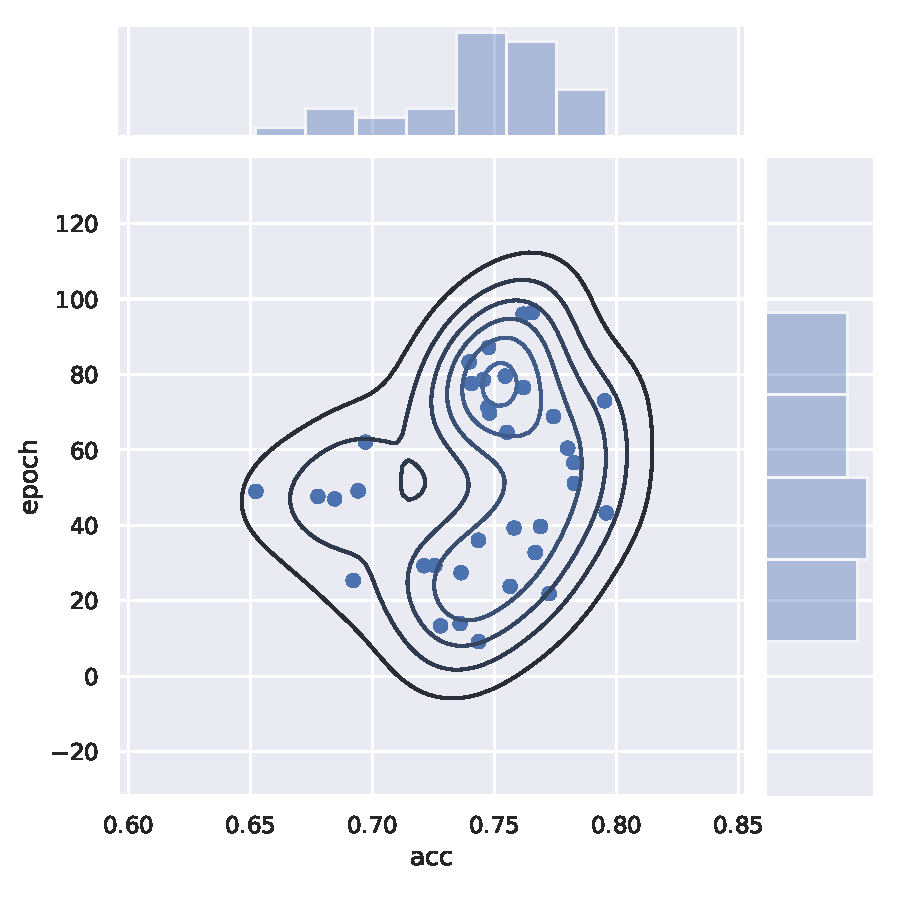
\includegraphics[scale=0.5]{anhang/GA_250_cifar10_False_big_jointplot_epoch.pdf}
  \caption{Dichte-Diagramm der Epochenanzahl in Verbindung mit der Klassifizierungsgenauigkeit(acc)}
\end{figure}

\begin{figure}[H]
  \centering  
  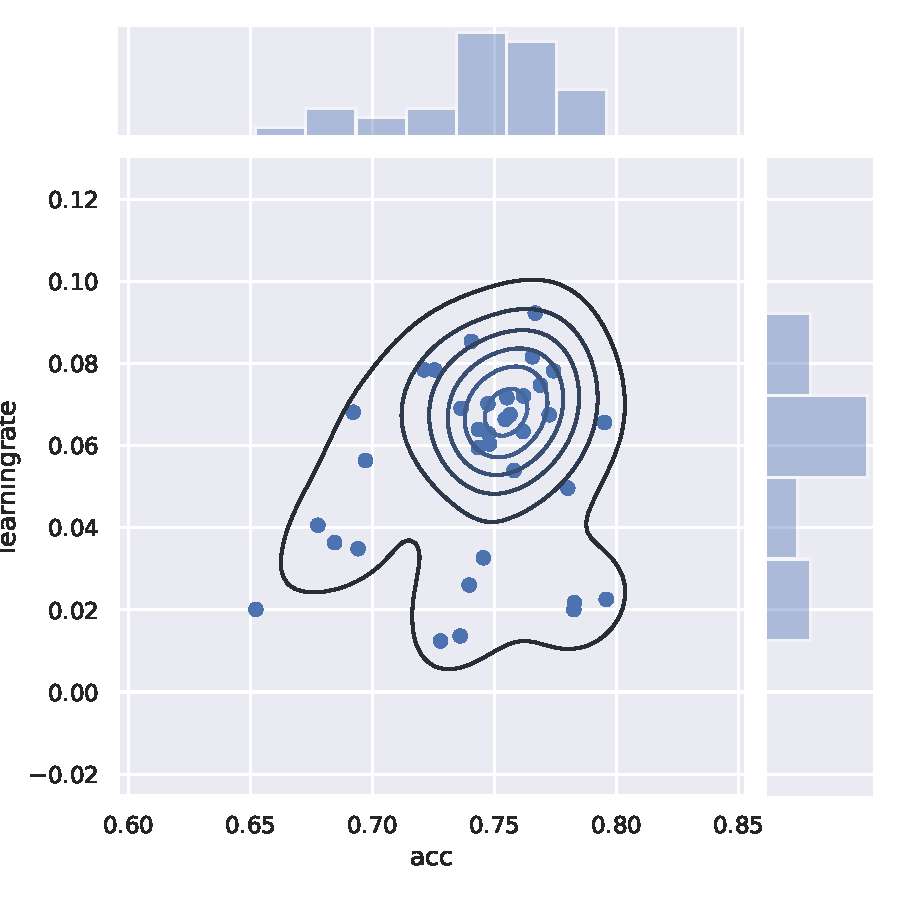
\includegraphics[scale=0.5]{anhang/GA_250_cifar10_False_big_jointplot_learningrate.pdf}
  \caption{Dichte-Diagramm der Lernrate in Verbindung mit der Klassifizierungsgenauigkeit(acc)}
\end{figure}

\begin{figure}[H]
  \centering  
  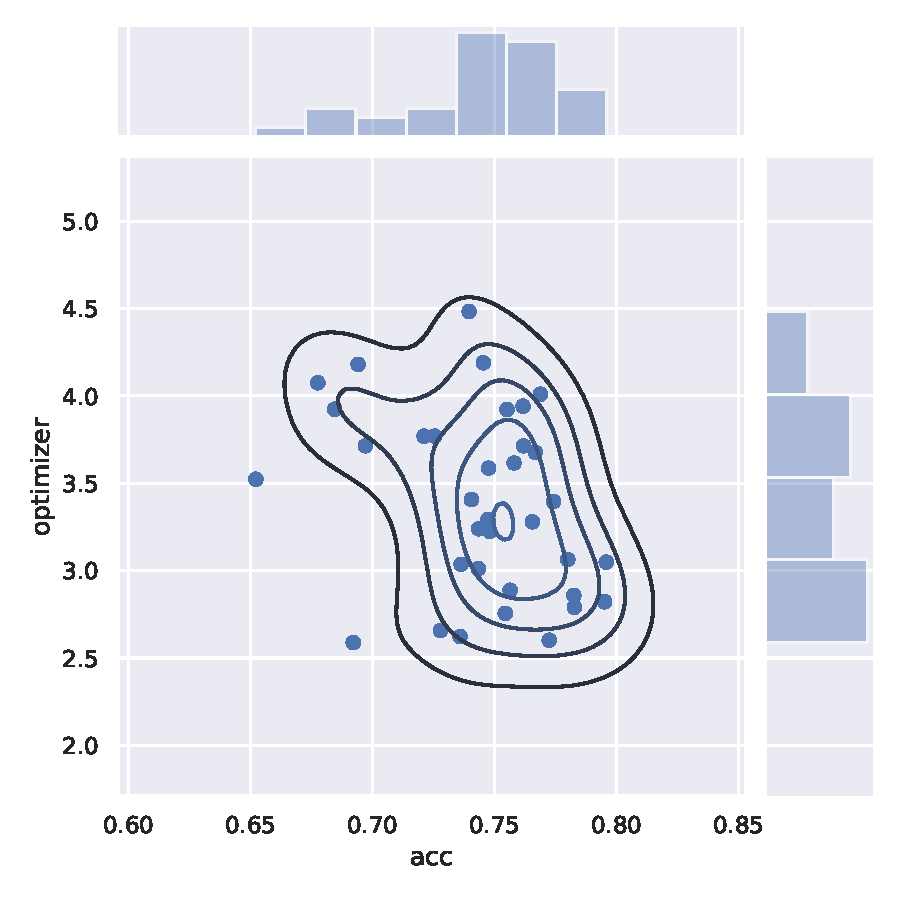
\includegraphics[scale=0.5]{anhang/GA_250_cifar10_False_big_jointplot_optimizer.pdf}
  \caption{Dichte-Diagramm des Optimierers in Verbindung mit der Klassifizierungsgenauigkeit(acc)}

\end{figure}



\section{Dichte-Diagramme zu den durchgeführten Optimierungen mit dem verkleinerten Datensatz}

\subsection{50 Iterationen des Genetischen Algorithmus des kleinen Fully-Connected Netzes}
\begin{figure}[H]
  \centering  
  \includegraphics[scale=0.5]{anhang/GA_50_mnist_digits_True_small_jointplot_batchsize.pdf}
  \caption{Dichte-Diagramm der Batchsize in Verbindung mit der Klassifizierungsgenauigkeit(acc)}
  
\end{figure}

\begin{figure}[H]
  \centering  
  \includegraphics[scale=0.5]{anhang/GA_50_mnist_digits_True_small_jointplot_dropout.pdf}
  \caption{Dichte-Diagramm des Dropouts in Verbindung mit der Klassifizierungsgenauigkeit(acc)}
  
\end{figure}

\begin{figure}[H]
  \centering  
  \includegraphics[scale=0.5]{anhang/GA_50_mnist_digits_True_small_jointplot_epoch.pdf}
  \caption{Dichte-Diagramm der Epochenanzahl in Verbindung mit der Klassifizierungsgenauigkeit(acc)}
  
\end{figure}

\begin{figure}[H]
  \centering  
  \includegraphics[scale=0.5]{anhang/GA_50_mnist_digits_True_small_jointplot_learningrate.pdf}
  \caption{Dichte-Diagramm der Lernrate in Verbindung mit der Klassifizierungsgenauigkeit(acc)}
  
\end{figure}

\begin{figure}[H]
  \centering  
  \includegraphics[scale=0.5]{anhang/GA_50_mnist_digits_True_small_jointplot_optimizer.pdf}
  \caption{Dichte-Diagramm der Optimierer in Verbindung mit der Klassifizierungsgenauigkeit(acc)}
  
\end{figure}

\subsection{50 Iterationen des Genetischen Algorithmus des großen Fully-Connected Netzes}
\begin{figure}[H]
  \centering  
  \includegraphics[scale=0.5]{anhang/GA_50_mnist_digits_True_big_jointplot_batchsize.pdf}
  \caption{Dichte-Diagramm der Batchsize in Verbindung mit der Klassifizierungsgenauigkeit(acc)}
  
\end{figure}

\begin{figure}[H]
  \centering  
  \includegraphics[scale=0.5]{anhang/GA_50_mnist_digits_True_big_jointplot_dropout.pdf}
  \caption{Dichte-Diagramm des Dropouts in Verbindung mit der Klassifizierungsgenauigkeit(acc)}
  
\end{figure}

\begin{figure}[H]
  \centering  
  \includegraphics[scale=0.5]{anhang/GA_50_mnist_digits_True_big_jointplot_epoch.pdf}
  \caption{Dichte-Diagramm der Epochenanzahl in Verbindung mit der Klassifizierungsgenauigkeit(acc)}
\end{figure}

\begin{figure}[H]
  \centering  
  \includegraphics[scale=0.5]{anhang/GA_50_mnist_digits_True_big_jointplot_learningrate.pdf}
  \caption{Dichte-Diagramm der Lernrate in Verbindung mit der Klassifizierungsgenauigkeit(acc)}
  
\end{figure}

\begin{figure}[H]
  \centering  
  \includegraphics[scale=0.5]{anhang/GA_50_mnist_digits_True_big_jointplot_optimizer.pdf}
  \caption{Dichte-Diagramm der Optimierer in Verbindung mit der Klassifizierungsgenauigkeit(acc)}
  
\end{figure}

\subsection{250 Iterationen des Genetischen Algorithmus des kleinen Fully-Connected Netzes}
\begin{figure}[H]
  \centering  
  \includegraphics[scale=0.5]{anhang/GA_250_mnist_digits_True_small_jointplot_batchsize.pdf}
  \caption{Dichte-Diagramm der Batchsize in Verbindung mit der Klassifizierungsgenauigkeit(acc)}
  
\end{figure}

\begin{figure}[H]
  \centering  
  \includegraphics[scale=0.5]{anhang/GA_250_mnist_digits_True_small_jointplot_dropout.pdf}
  \caption{Dichte-Diagramm des Dropouts in Verbindung mit der Klassifizierungsgenauigkeit(acc)}
  
\end{figure}

\begin{figure}[H]
  \centering  
  \includegraphics[scale=0.5]{anhang/GA_250_mnist_digits_True_small_jointplot_epoch.pdf}
  \caption{Dichte-Diagramm der Epochenanzahl in Verbindung mit der Klassifizierungsgenauigkeit(acc)}
  
\end{figure}

\begin{figure}[H]
  \centering  
  \includegraphics[scale=0.5]{anhang/GA_250_mnist_digits_True_small_jointplot_learningrate.pdf}
  \caption{Dichte-Diagramm der Lernrate in Verbindung mit der Klassifizierungsgenauigkeit(acc)}
  
\end{figure}

\begin{figure}[H]
  \centering  
  \includegraphics[scale=0.5]{anhang/GA_250_mnist_digits_True_small_jointplot_optimizer.pdf}
  \caption{Dichte-Diagramm der Optimierer in Verbindung mit der Klassifizierungsgenauigkeit(acc)}
  
\end{figure}


\subsection{250 Iterationen des Genetischen Algorithmus des großen Fully-Connected Netzes}
\begin{figure}[H]
  \centering  
  \includegraphics[scale=0.5]{anhang/GA_250_mnist_digits_True_big_jointplot_batchsize.pdf}
  \caption{Dichte-Diagramm der Batchsize in Verbindung mit der Klassifizierungsgenauigkeit(acc)}
  
\end{figure}

\begin{figure}[H]
  \centering  
  \includegraphics[scale=0.5]{anhang/GA_250_mnist_digits_True_big_jointplot_dropout.pdf}
  \caption{Dichte-Diagramm des Dropouts in Verbindung mit der Klassifizierungsgenauigkeit(acc)}
  
\end{figure}

\begin{figure}[H]
  \centering  
  \includegraphics[scale=0.5]{anhang/GA_250_mnist_digits_True_big_jointplot_epoch.pdf}
  \caption{Dichte-Diagramm der Epochenanzahl in Verbindung mit der Klassifizierungsgenauigkeit(acc)}
  
\end{figure}

\begin{figure}[H]
  \centering  
  \includegraphics[scale=0.5]{anhang/GA_250_mnist_digits_True_big_jointplot_learningrate.pdf}
  \caption{Dichte-Diagramm der Lernrate in Verbindung mit der Klassifizierungsgenauigkeit(acc)}
  
\end{figure}

\begin{figure}[H]
  \centering  
  \includegraphics[scale=0.5]{anhang/GA_250_mnist_digits_True_big_jointplot_optimizer.pdf}
  \caption{Dichte-Diagramm der Optimierer in Verbindung mit der Klassifizierungsgenauigkeit(acc)}
  
\end{figure}

\subsection{50 Iterationen des Genetischen Algorithmus des Convolutional Neural Network}
\begin{figure}[H]
  \centering  
  \includegraphics[scale=0.5]{anhang/GA_50_cifar10_True_big_jointplot_batchsize.pdf}
  \caption{Dichte-Diagramm der Batchsize in Verbindung mit der Klassifizierungsgenauigkeit(acc)}
  
\end{figure}

\begin{figure}[H]
  \centering  
  \includegraphics[scale=0.5]{anhang/GA_50_cifar10_True_big_jointplot_dropout.pdf}
  \caption{Dichte-Diagramm des Dropouts in Verbindung mit der Klassifizierungsgenauigkeit(acc)}
  
\end{figure}

\begin{figure}[H]
  \centering  
  \includegraphics[scale=0.5]{anhang/GA_50_cifar10_True_big_jointplot_epoch.pdf}
  \caption{Dichte-Diagramm der Epochenanzahl in Verbindung mit der Klassifizierungsgenauigkeit(acc)}
  
\end{figure}

\begin{figure}[H]
  \centering  
  \includegraphics[scale=0.5]{anhang/GA_50_cifar10_True_big_jointplot_learningrate.pdf}
  \caption{Dichte-Diagramm der Lernrate in Verbindung mit der Klassifizierungsgenauigkeit(acc)}
  
\end{figure}

\begin{figure}[H]
  \centering  
  \includegraphics[scale=0.5]{anhang/GA_50_cifar10_True_big_jointplot_optimizer.pdf}
  \caption{Dichte-Diagramm des Optimierers in Verbindung mit der Klassifizierungsgenauigkeit(acc)}
  
\end{figure}

\subsection{250 Iterationen des Genetischen Algorithmus des Convolutional Neural Network}
\begin{figure}[H]
  \centering  
  \includegraphics[scale=0.5]{anhang/GA_250_cifar10_True_big_jointplot_batchsize.pdf}
  \caption{Dichte-Diagramm der Batchsize in Verbindung mit der Klassifizierungsgenauigkeit(acc)}
  
\end{figure}

\begin{figure}[H]
  \centering  
  \includegraphics[scale=0.5]{anhang/GA_250_cifar10_True_big_jointplot_dropout.pdf}
  \caption{Dichte-Diagramm des Dropouts in Verbindung mit der Klassifizierungsgenauigkeit(acc)}
  
\end{figure}

\begin{figure}[H]
  \centering  
  \includegraphics[scale=0.5]{anhang/GA_250_cifar10_True_big_jointplot_epoch.pdf}
  \caption{Dichte-Diagramm der Epochenanzahl in Verbindung mit der Klassifizierungsgenauigkeit(acc)}
  
\end{figure}

\begin{figure}[H]
  \centering  
  \includegraphics[scale=0.5]{anhang/GA_250_cifar10_True_big_jointplot_learningrate.pdf}
  \caption{Dichte-Diagramm der Lernrate in Verbindung mit der Klassifizierungsgenauigkeit(acc)}
  
\end{figure}

\begin{figure}[H]
  \centering  
  \includegraphics[scale=0.5]{anhang/GA_250_cifar10_True_big_jointplot_optimizer.pdf}
  \caption{Dichte-Diagramm des Optimierers in Verbindung mit der Klassifizierungsgenauigkeit(acc)}
  
\end{figure}
\cleardoublepage

\newpage
%Verzeichnis aller Bilder
\listoffigures



\end{document}
